% ============================================================
%  ANI Coral Reef Research Report
%  Step-by-step accumulation — Phase 1: EDA & Feature Analysis
% ============================================================
\documentclass[12pt,a4paper]{report}

% ── Packages ─────────────────────────────────────────────────
\usepackage[margin=2.5cm]{geometry}
\usepackage{amsmath,amssymb}
\usepackage[T1]{fontenc}
\usepackage[utf8]{inputenc}
\usepackage{lmodern}
\usepackage{booktabs}
\usepackage{longtable}
\usepackage{array}
\usepackage{multirow}
\usepackage{graphicx}
\usepackage{float}
\usepackage[table,xcdraw]{xcolor}
\usepackage{hyperref}
\usepackage{caption}
\usepackage{subcaption}
\usepackage{enumitem}
\usepackage{titlesec}
\usepackage{fancyhdr}
\usepackage{parskip}
\usepackage{microtype}
\usepackage{mdframed}

% ── Colours ──────────────────────────────────────────────────
\definecolor{darkblue}{RGB}{0,51,102}
\definecolor{medblue}{RGB}{0,90,160}
\definecolor{lightblue}{RGB}{173,216,230}
\definecolor{darkgreen}{RGB}{0,100,0}
\definecolor{lightgreen}{RGB}{144,238,144}
\definecolor{orange}{RGB}{255,140,0}
\definecolor{red}{RGB}{180,0,0}
\definecolor{rowgray}{RGB}{245,245,245}

% ── Section formatting ────────────────────────────────────────
\titleformat{\chapter}[block]
  {\normalfont\Huge\bfseries\color{darkblue}}
  {\thechapter.}{1em}{}
\titleformat{\section}
  {\normalfont\Large\bfseries\color{medblue}}
  {\thesection}{1em}{}
\titleformat{\subsection}
  {\normalfont\large\bfseries\color{darkblue!70}}
  {\thesubsection}{1em}{}

% ── Header / Footer ───────────────────────────────────────────
\pagestyle{fancy}
\fancyhf{}
\fancyhead[L]{\small\textcolor{darkblue}{ANI Coral Reef Research — Independent Study}}
\fancyhead[R]{\small\textcolor{darkblue}{\nouppercase{\leftmark}}}
\fancyfoot[C]{\thepage}
\renewcommand{\headrulewidth}{0.4pt}

% ── Hyperref setup ────────────────────────────────────────────
\hypersetup{
  colorlinks=true,
  linkcolor=medblue,
  urlcolor=medblue,
  citecolor=darkgreen,
  pdftitle={ANI Coral Reef Research Report},
  pdfauthor={Independent Study}
}

% ── Custom box environments ───────────────────────────────────
\newmdenv[linecolor=medblue,linewidth=1.5pt,backgroundcolor=lightblue!20,
  innerleftmargin=8pt,innerrightmargin=8pt,innertopmargin=6pt,innerbottommargin=6pt]{infobox}

\newmdenv[linecolor=darkgreen,linewidth=1.5pt,backgroundcolor=lightgreen!20,
  innerleftmargin=8pt,innerrightmargin=8pt,innertopmargin=6pt,innerbottommargin=6pt]{findingbox}

\newmdenv[linecolor=orange,linewidth=1.5pt,backgroundcolor=orange!10,
  innerleftmargin=8pt,innerrightmargin=8pt,innertopmargin=6pt,innerbottommargin=6pt]{challengebox}

% ── Column types ─────────────────────────────────────────────
\newcolumntype{L}[1]{>{\raggedright\arraybackslash}p{#1}}
\newcolumntype{C}[1]{>{\centering\arraybackslash}p{#1}}
\newcolumntype{R}[1]{>{\raggedleft\arraybackslash}p{#1}}

% =============================================================
\begin{document}

% ── Title Page ───────────────────────────────────────────────
\begin{titlepage}
  \centering
  \vspace*{2cm}
  {\color{darkblue}\rule{\linewidth}{2pt}}\\[0.4cm]
  {\Huge\bfseries\color{darkblue}
    Coral Reef Monitoring and Prediction\\[0.3cm]
    in the Andaman \& Nicobar Islands\\[0.3cm]
    Using Satellite Remote Sensing and ML}\\[0.4cm]
  {\color{darkblue}\rule{\linewidth}{2pt}}\\[1.5cm]

  {\Large\bfseries\color{medblue} Independent Study Report}\\[0.3cm]
  {\large Phases 1--3: EDA, Water Quality Prediction, Bleaching Early Warning, and Global Climate Analysis}\\[2cm]

  \begin{tabular}{ll}
    \textbf{Datasets} & Andaman 20-Year (2004--2024), Harmonized, Global \\[4pt]
    \textbf{Data Source} & MODIS Aqua (COPERNICUS V6), ERA5 (ECMWF) via GEE \\[4pt]
    \textbf{Reef Sites} & Havelock, Neil, Port Blair, Wandoor (ANI) \\[4pt]
    \textbf{Date} & March 2026 \\
  \end{tabular}

  \vfill
  {\footnotesize
    All three research tasks have been completed and are documented in this report,\\
    along with a final Conclusion chapter synthesising findings across all tasks.}
\end{titlepage}

% ── Table of Contents ─────────────────────────────────────────
\tableofcontents
\clearpage

% =============================================================
\chapter{Introduction and Problem Statements}
% =============================================================

\section{Research Context}

The Andaman and Nicobar Islands (ANI), located in the northeastern Indian Ocean, host
some of India's most ecologically significant coral reef systems. Spanning approximately
2,000 km$^2$ of shallow tropical waters, these reefs support extraordinary biodiversity
and provide livelihoods for thousands of island communities. Yet they face escalating
pressures from ocean warming, monsoon-driven runoff, and climate variability. Despite
their ecological importance, ANI reefs remain severely under-studied in the context of
data-driven, satellite-based monitoring.

Existing monitoring frameworks rely on periodic scuba-dive surveys and a handful of
permanent oceanographic buoys. This makes continuous, real-time or predictive assessment
impractical. The emergence of freely available satellite products — MODIS Aqua ocean
colour (NASA's Earth-observing satellite that measures ocean properties from space),
ERA5 reanalysis (a global hourly reconstruction of weather and ocean conditions produced
by the European Centre for Medium-Range Weather Forecasts), and Copernicus Marine Service
datasets — offers an unprecedented opportunity to replace expensive field campaigns with
long-term, automated monitoring systems that can detect reef stress before it is visible
to a diver.

This study addresses three inter-linked research tasks that together form a satellite-driven
reef health monitoring pipeline for ANI.

\section{Research Tasks}

\subsection*{Task 1 — Coral Reef Water Quality Prediction (Primary ML Task)}

\begin{infobox}
\textbf{Problem:} ANI reefs lack any predictive water quality modelling.\\[4pt]
\textbf{Approach:} Combine satellite and atmospheric data — MODIS Aqua chlorophyll
(\texttt{chlor\_a}, the concentration of photosynthetic pigment in the water, used as a
proxy for algal growth and water clarity), engineered turbidity (derived from
Rrs$_{443}$, Rrs$_{490}$ — satellite reflectance values at two blue-light wavelengths
that reveal how murky or clear the water is), sea surface temperature (SST — the
temperature at the top of the ocean), and ERA5 wind-derived wave energy — into a
weekly water quality prediction model.\\[4pt]
\textbf{Target:} Predict next week's chlorophyll-$a$ concentration (\texttt{chlor\_a}$_{t+1}$).\\ 
Higher chlorophyll means more algal growth, which can cloud the water and stress corals.\\[4pt]
\textbf{Models:} Random Forest (baseline) and XGBoost (primary) — both are powerful
tree-based machine learning algorithms that combine many simple decision rules to make
accurate predictions — evaluated with time-series cross-validation (a method that
ensures the model is always tested on future data it has never seen, preventing
artificially inflated accuracy scores).
\end{infobox}

\subsection*{Task 2 — Coral Bleaching Early Warning Index (Secondary — Andaman Only)}

\begin{infobox}
\textbf{Full Title:} A Satellite-Derived Early Warning System for Coral Bleaching in ANI
Reefs Using Sea Surface Temperature and Ocean Colour Anomalies.\\[4pt]
\textbf{Approach:} Compute weekly SST anomalies against the 20-year site-level climatology
to derive a Degree Heating Week (DHW) proxy. Combine with \texttt{chlor\_a} and light
attenuation anomalies to produce a composite bleaching stress index.\\[4pt]
\textbf{Output:} Weekly risk score (0--1) per reef site; threshold-based alert levels.
\end{infobox}

\subsection*{Task 3 — Global and Andaman Climate Change Linkage}

\begin{infobox}
\textbf{Approach:} Compare long-term SST and chlorophyll trends across 6 global reef sites
(Great Barrier Reef, Florida, Red Sea, Seychelles, Mediterranean, Hawaii) and the 4 ANI
sites.\\[4pt]
\textbf{Methods:} Mann-Kendall trend tests (a statistical method for detecting whether
a variable — such as temperature — is consistently rising or falling over many years,
even with noisy data), Sen's slope (the median rate of change per year), and
cross-correlation with major climate indices:\\[4pt]
\quad\textit{ENSO} = El Ni\~no-Southern Oscillation — the periodic warming (El Ni\~no)
and cooling (La Ni\~na) of the central Pacific Ocean that disrupts global weather
patterns every 2--7 years.\\[2pt]
\quad\textit{IOD} = Indian Ocean Dipole — an analogous see-saw pattern specific to
the Indian Ocean, in which one side warms while the other cools, strongly affecting
rainfall and ocean temperatures across South and Southeast Asia.\\[4pt]
\textbf{Question:} Is the ANI reef SST warming trend consistent with global patterns,
and is there a measurable accelerating trend in bleaching-level stress?
\end{infobox}

\section{Datasets Summary}

\begin{table}[H]
\centering
\caption{Overview of datasets used in this study}
\begin{tabular}{L{3.5cm}L{3cm}C{1.8cm}C{1.8cm}L{4cm}}
\toprule
\textbf{Dataset} & \textbf{Scope} & \textbf{Period} & \textbf{Rows} & \textbf{Key Columns} \\
\midrule
\rowcolor{rowgray}
Andaman 20-Year & 4 reef sites, weekly & 2004--2024 & 4,380 & chlor\_a, SST, precip, total\_nobs \\
Andaman Harmonized & 4 reef sites, weekly & 2004--2024 & 4,380 & + Rrs\_443/490, u\_wind, v\_wind, mslp \\
\rowcolor{rowgray}
Global 20-Year & 6 reef sites, monthly & 2004--2024 & $\sim$1,440 & chlor\_a, SST, precip \\
Global Harmonized & 6 reef sites, monthly & 2004--2024 & $\sim$1,440 & + Rrs\_443/490, u\_wind, v\_wind, mslp \\
\bottomrule
\end{tabular}
\label{tab:datasets}
\end{table}

\textbf{Data source:} Google Earth Engine — COPERNICUS/MARINE/SATELLITE\_OCEAN\_COLOR/V6
(MODIS Aqua) for ocean colour bands; ECMWF/ERA5/HOURLY for atmospheric and
surface variables. All composited at weekly (Andaman) or monthly (Global) resolution
using spatial mean reduction over 5 km (Andaman) and 10 km (Global) reef buffers.

\subsection*{Data Availability}

All four datasets are publicly available for download via Google Drive:

\begin{table}[H]
\centering
\caption{Dataset download links}
\begin{tabular}{L{5cm}L{9cm}}
\toprule
\textbf{File} & \textbf{Download Link} \\
\midrule
\rowcolor{rowgray}
\texttt{Andaman\_WQ\_20Year\_Dataset.csv} &
  \url{https://drive.google.com/file/d/1xGrP9394_Lg2NX7RWA_SYin6TfJhS7oI/view?usp=sharing} \\
\texttt{Andaman\_WQ\_Harmonized\_20Year.csv} &
  \url{https://drive.google.com/file/d/1NuzkKS2m6Ty6NRpRbLWFab7rH2xpjtYv/view?usp=sharing} \\
\rowcolor{rowgray}
\texttt{Global\_WQ\_20Year\_Dataset.csv} &
  \url{https://drive.google.com/file/d/1Nw-FA1BSg3Y1cLlm8afrZNV2TLAJqshW/view?usp=sharing} \\
\texttt{Global\_WQ\_Harmonized\_20Year.csv} &
  \url{https://drive.google.com/file/d/1f3x0m_zkJoSmg4C7MP69TF5LIfXdaTs1/view?usp=sharing} \\
\bottomrule
\end{tabular}
\label{tab:dataset_links}
\end{table}

\subsection*{Code Availability}

All analysis notebooks, the LaTeX report source, and supporting scripts are
publicly available at:

\begin{center}
  \url{https://github.com/MuditGupta2502/andaman-reef-monitoring}
\end{center}

% =============================================================
\chapter{Exploratory Data Analysis}
% =============================================================

\section{Dataset Structure and Completeness}

\subsection{Andaman 20-Year Dataset}

\begin{table}[H]
\centering
\caption{Column-level profile — Andaman 20-Year Dataset (4,380 rows $\times$ 8 columns)}
\begin{tabular}{L{4.5cm}C{2cm}R{1.8cm}R{1.8cm}R{2cm}}
\toprule
\textbf{Column} & \textbf{Type} & \textbf{Non-null} & \textbf{Missing} & \textbf{Missing \%} \\
\midrule
\rowcolor{rowgray}
chlor\_a & float64 & 2,779 & 1,601 & \textcolor{red}{\textbf{36.55\%}} \\
total\_nobs & float64 & 2,779 & 1,601 & \textcolor{red}{\textbf{36.55\%}} \\
\rowcolor{rowgray}
sea\_surface\_temperature & float64 & 4,380 & 0 & \textcolor{darkgreen}{0.00\%} \\
total\_precipitation & float64 & 4,380 & 0 & \textcolor{darkgreen}{0.00\%} \\
\rowcolor{rowgray}
label & string & 4,380 & 0 & \textcolor{darkgreen}{0.00\%} \\
week\_start & string & 4,380 & 0 & \textcolor{darkgreen}{0.00\%} \\
\bottomrule
\end{tabular}
\label{tab:profile_20y}
\end{table}

\begin{findingbox}
\textbf{Finding:} The 36.55\% missingness in \texttt{chlor\_a} and \texttt{total\_nobs}
is expected and non-random. MODIS Aqua is an optical sensor — cloud cover during the
SW monsoon (June--September) and cloud contamination in the tropical belt systematically
prevent valid retrievals. This missingness carries information and must be handled via
site-level linear interpolation with a maximum gap limit (e.g., 4 weeks) before modelling.
\end{findingbox}

\subsection{Andaman Harmonized Dataset}

\begin{table}[H]
\centering
\caption{Column-level profile — Andaman Harmonized Dataset (4,380 rows $\times$ 13 columns)}
\begin{tabular}{L{4.5cm}C{2cm}R{1.8cm}R{1.8cm}R{2cm}}
\toprule
\textbf{Column} & \textbf{Type} & \textbf{Non-null} & \textbf{Missing} & \textbf{Missing \%} \\
\midrule
\rowcolor{rowgray}
chlor\_a & float64 & 2,779 & 1,601 & \textcolor{red}{\textbf{36.55\%}} \\
Rrs\_443 & float64 & 2,779 & 1,601 & \textcolor{red}{\textbf{36.55\%}} \\
\rowcolor{rowgray}
Rrs\_490 & float64 & 2,779 & 1,601 & \textcolor{red}{\textbf{36.55\%}} \\
total\_nobs & float64 & 2,779 & 1,601 & \textcolor{red}{\textbf{36.55\%}} \\
\rowcolor{rowgray}
sst & float64 & 4,380 & 0 & \textcolor{darkgreen}{0.00\%} \\
precip & float64 & 4,380 & 0 & \textcolor{darkgreen}{0.00\%} \\
\rowcolor{rowgray}
u\_wind & float64 & 4,380 & 0 & \textcolor{darkgreen}{0.00\%} \\
v\_wind & float64 & 4,380 & 0 & \textcolor{darkgreen}{0.00\%} \\
\rowcolor{rowgray}
mslp & float64 & 4,380 & 0 & \textcolor{darkgreen}{0.00\%} \\
\bottomrule
\end{tabular}
\label{tab:profile_harm}
\end{table}

\begin{findingbox}
\textbf{Finding:} All MODIS-derived bands (\texttt{chlor\_a}, \texttt{Rrs\_443},
\texttt{Rrs\_490}, \texttt{total\_nobs}) share identical missingness patterns — they are
absent together whenever cloud cover prevents valid pixel retrieval. ERA5-derived variables
have zero missing values as they are reanalysis products (model-based, not observation-dependent).
\end{findingbox}

\section{Descriptive Statistics}

\begin{table}[H]
\centering
\caption{Descriptive statistics — key numeric variables}
\begin{tabular}{L{4.2cm}R{1.5cm}R{1.5cm}R{1.5cm}R{1.5cm}R{1.5cm}R{1.5cm}}
\toprule
\textbf{Variable} & \textbf{Mean} & \textbf{Std} & \textbf{Min} & \textbf{25\%} & \textbf{Median} & \textbf{Max} \\
\midrule
\rowcolor{rowgray}
chlor\_a (mg m$^{-3}$) & 0.560 & 0.314 & 0.137 & 0.352 & 0.460 & 2.588 \\
SST (K) & 302.08 & 0.821 & 300.14 & 301.50 & 301.97 & 305.14 \\
\rowcolor{rowgray}
SST ($^\circ$C) & 28.93 & 0.82 & 26.99 & 28.35 & 28.82 & 31.99 \\
precip (m day$^{-1}$) & 0.0003 & 0.0003 & 0 & 0 & 0.0002 & 0.0017 \\
\rowcolor{rowgray}
u\_wind (m s$^{-1}$) & 0.77 & 4.40 & $-8.16$ & $-3.10$ & $-0.11$ & 8.81 \\
v\_wind (m s$^{-1}$) & 1.02 & 3.44 & $-5.71$ & $-2.05$ & 0.51 & 10.03 \\
\rowcolor{rowgray}
mslp (Pa) & 100,956 & 209 & 100,337 & 100,796 & 100,950 & 101,565 \\
\bottomrule
\end{tabular}
\label{tab:stats}
\end{table}

\textbf{Site balance:} Each of the four reef sites (Port Blair, Havelock, Neil, Wandoor)
contributes exactly 1,095 weekly records — the dataset is perfectly balanced, which
eliminates site-level sampling bias from modelling.

\section{Key EDA Findings by Variable}

\subsection{Chlorophyll-a (\texttt{chlor\_a})}

\begin{itemize}[leftmargin=*]
  \item \textbf{Distribution:} Strongly right-skewed — meaning most weeks record
    moderate values near 0.46 mg\,m$^{-3}$, but occasional monsoon bloom events push
    concentrations to 2.59 mg\,m$^{-3}$, over five times the typical baseline.
    The mean (0.56) exceeds the median (0.46) precisely because of these rare but
    intense spikes — a common pattern in natural phenomena like rainfall or river flow.
  \item \textbf{Seasonality:} Clear bimodal pattern — elevated values in June--July
    (SW monsoon onset, upwelling-driven nutrient input) and a secondary peak in
    February--March (NE monsoon stirring).
  \item \textbf{Relevance to Task 1:} This is the primary prediction target. Its
    right-skewed distribution suggests a log-transform prior to regression targets
    may improve model residual normality.
  \item \textbf{Relevance to Task 2:} Positive anomalies above the site-month
    climatological mean can indicate turbidity/nutrient stress co-occurring with
    thermal bleaching stress; negative anomalies during warm periods may signal
    prior bleaching mortality of zooxanthellae.
\end{itemize}

\subsection{Sea Surface Temperature (SST)}

\begin{itemize}[leftmargin=*]
  \item \textbf{Distribution:} Near-normal, centred at 28.93$^\circ$C (302.08 K),
    range 26.99--31.99$^\circ$C.
  \item \textbf{Seasonality:} Strong unimodal peak in April--May (pre-monsoon solar
    heating). Rapid cooling begins in June as the SW monsoon brings cloud cover and
    upwelling. Minimum values in January--February(NE monsoon).
  \item \textbf{Critical threshold:} The tropical bleaching threshold is typically
    defined as $\geq$1$^\circ$C above the maximum monthly mean (MMM). With MMM
    $\approx$ 30.5$^\circ$C (April), observations above 31.5$^\circ$C constitute
    bleaching-level thermal stress. The dataset max of 31.99$^\circ$C confirms that
    bleaching-threshold events have occurred at ANI.
  \item \textbf{Relevance to Task 2:} Baseline climatology (mean SST per site per
    calendar month) will be computed from the full 20-year record to derive weekly
    anomalies (SST$_{\text{anomaly}}$ = SST$_t$ $-$ SST$_{\text{climatology}}$).
  \item \textbf{Relevance to Task 3:} The most important variable for global
    comparative warming trend analysis.
\end{itemize}

\subsection{Wind Components and Wave Energy Proxy}

\begin{itemize}[leftmargin=*]
  \item \textbf{u\_wind:} East-west component, mean near zero, bimodal distribution
    reflecting monsoon reversal (positive/eastward in NE monsoon; negative/westward
    in SW monsoon).
  \item \textbf{v\_wind:} North-south component, mean slightly positive (1.02 m\,s$^{-1}$),
    reflecting the net southerly-to-northerly flow that characterises the Bay of Bengal.
  \item \textbf{Wave energy proxy:} $E_{\text{wave}} = u_{\text{wind}}^2 + v_{\text{wind}}^2$
    (proportional to kinetic energy per unit mass). This is the ERA5-based proxy for
    wave energy in the absence of direct wave spectral data.
  \item \textbf{Relevance to Task 1:} Wave energy drives sediment resuspension and
    turbidity — a known driver of \texttt{chlor\_a} variability in shallow reef systems.
\end{itemize}

\subsection{Reflectance Bands (Rrs\_443, Rrs\_490)}

\begin{itemize}[leftmargin=*]
  \item \textbf{Purpose:} These are MODIS satellite measurements of how strongly
    the ocean surface reflects sunlight at two blue-light wavelengths: 443\,nm (blue)
    and 490\,nm (blue-green). Together they are used to derive the diffuse attenuation
    coefficient $K_d(490)$ — a measure of how quickly sunlight dims as it travels
    deeper into the water, which serves as the primary proxy for turbidity (water
    cloudiness) and light availability at the coral surface.
  \item \textbf{Engineering formula:}
    $K_{d,\text{proxy}} = 0.0232 + 0.2 \times (\text{Rrs}_{490} - \text{Rrs}_{443})$
    (empirical approximation after Lee et al.\ 2005).
  \item \textbf{Missingness:} Identical to \texttt{chlor\_a} (36.55\%) — all MODIS
    optical bands fail simultaneously under clouds.
  \item \textbf{Relevance to Task 1 \& 2:} $K_d$ will serve as the turbidity feature
    replacing any placeholder; also used as a bleaching stress modifier in Task 2
    (high turbidity can provide thermal refuge or indicate sedimentation stress).
\end{itemize}

\section{Correlation Analysis}

\begin{table}[H]
\centering
\caption{Pairwise Pearson correlations among key numeric variables (Harmonized dataset). Pearson correlation ($r$) ranges from $-1$ (perfect inverse relationship: as one variable rises, the other falls) through 0 (no linear association) to $+1$ (perfect positive relationship). Values between $\pm$0.1 and $\pm$0.3 are considered weak but non-trivial.}
\begin{tabular}{L{3.5cm}R{2cm}R{2cm}R{2cm}R{2cm}}
\toprule
 & \textbf{chlor\_a} & \textbf{sst} & \textbf{u\_wind} & \textbf{v\_wind} \\
\midrule
\rowcolor{rowgray}
chlor\_a & 1.00 & $-$0.16 & --- & --- \\
sst     & $-$0.16 & 1.00 & --- & --- \\
\rowcolor{rowgray}
u\_wind  & --- & --- & 1.00 & --- \\
v\_wind  & --- & --- & --- & 1.00 \\
\bottomrule
\end{tabular}
\label{tab:corr}
\end{table}

\begin{findingbox}
\textbf{chlor\_a vs.\ SST = $-$0.16:} Weak negative correlation at the raw weekly
level. This reflects a biological and physical mechanism: the SW monsoon simultaneously
cools the sea surface via upwelling and increases nutrient supply, driving chlorophyll
up. However, the raw site-pooled correlation is diluted by inter-site and seasonal
variability. Per-site, per-season correlations are expected to be substantially stronger
and will be computed in the modelling phase.
\end{findingbox}

\section{Temporal Coverage and Reef Site Balance}

\begin{itemize}[leftmargin=*]
  \item \textbf{Date range:} 2004-01-01 to 2024-12-19 (20 years, weekly resolution,
    1,095 unique weeks).
  \item \textbf{Site counts:} Each of Port Blair, Havelock, Neil, and Wandoor contributes
    exactly 1,095 rows — perfect balance, no site-level upsampling needed.
  \item \textbf{Geographic spread:}
    \begin{itemize}
      \item \textit{Havelock \& Neil:} Mid-ocean, exposed oceanic reefs — lower
        turbidity baseline, more sensitive to thermal bleaching.
      \item \textit{Port Blair \& Wandoor:} Near-shore, influenced by terrestrial
        runoff and sedimentation — higher chlorophyll baseline, more nutrient-stressed.
    \end{itemize}
  \item This site heterogeneity motivates per-site sub-models (or site as a
    categorical feature) rather than a single pooled model.
\end{itemize}

% =============================================================
\chapter{Feature Analysis for Each Research Task}
% =============================================================

\section{Feature Availability and Engineering Plan}

\begin{table}[H]
\centering
\caption{Feature availability and engineering plan across all three tasks}
\begin{tabular}{L{3.2cm}C{1.4cm}C{1.4cm}C{1.4cm}L{4.5cm}}
\toprule
\textbf{Feature} & \textbf{Task 1 (Water Quality)} & \textbf{Task 2 (Bleaching)} & \textbf{Task 3 (Climate)} & \textbf{Status / Action} \\
\midrule
\rowcolor{rowgray}
\texttt{chlor\_a} & Target (t+1) & Anomaly & Trend & \textcolor{darkgreen}{Direct — available} \\
SST & Feature & Anomaly & Trend & \textcolor{darkgreen}{Direct — available} \\
\rowcolor{rowgray}
\texttt{precip} & Feature & --- & --- & \textcolor{darkgreen}{Direct — available} \\
\texttt{u\_wind}, \texttt{v\_wind} & Feature & --- & --- & \textcolor{darkgreen}{Available (ERA5)} \\
\rowcolor{rowgray}
\texttt{mslp} & Feature & --- & --- & \textcolor{darkgreen}{Available (ERA5)} \\
\texttt{Rrs\_443}, \texttt{Rrs\_490} & Feature & Feature & --- & \textcolor{darkgreen}{Available (MODIS)} \\
\rowcolor{rowgray}
Turbidity ($K_d$ proxy) & Feature & Feature & --- & \textcolor{orange}{\textbf{Engineer}} from Rrs bands \\
Wave energy ($E_w$) & Feature & --- & --- & \textcolor{orange}{\textbf{Engineer}} $= u^2 + v^2$ \\
\rowcolor{rowgray}
SST anomaly & --- & Target/Feat. & Input & \textcolor{orange}{\textbf{Engineer}} vs.\ 20-yr climatology \\
DHW proxy & --- & Index & --- & \textcolor{orange}{\textbf{Engineer}} cumulative SST excess \\
\rowcolor{rowgray}
Lag features (t$-$1, t$-$2, t$-$4) & Feature & --- & --- & \textcolor{orange}{\textbf{Engineer}} time-shift \\
Seasonal features (sin/cos month) & Feature & Feature & --- & \textcolor{orange}{\textbf{Engineer}} cyclic encoding \\
\rowcolor{rowgray}
Site encoding & Feature & Feature & --- & \textcolor{orange}{\textbf{Engineer}} label-encode \\
Mann-Kendall slope & --- & --- & Output & Computed during Task 3 \\
\bottomrule
\end{tabular}
\label{tab:features}
\end{table}

\section{Task 1 — Feature Engineering Detail}

For the water quality prediction model, the final feature matrix will be constructed as
follows:

\begin{enumerate}[leftmargin=*]
  \item \textbf{Imputation:} \texttt{chlor\_a} (and all MODIS bands) will be imputed per
    site using linear interpolation with a maximum gap of 4 consecutive weeks; longer gaps
    remain NaN and those rows will be excluded from training.
  \item \textbf{Derived features:}
    \begin{align}
      K_{d,\text{proxy}} &= 0.0232 + 0.2 \times (\text{Rrs}_{490} - \text{Rrs}_{443}) \\
      E_{\text{wave}} &= u_{\text{wind}}^2 + v_{\text{wind}}^2 \\
      \text{chlor\_a\_log} &= \log(1 + \text{chlor\_a})
    \end{align}
  \item \textbf{Lag features:} \texttt{chlor\_a}$_{t-1}$, \texttt{chlor\_a}$_{t-2}$,
    \texttt{chlor\_a}$_{t-4}$, \texttt{SST}$_{t-1}$, $E_{\text{wave},t-1}$
  \item \textbf{Cyclic encoding:}
    \begin{align}
      \text{month\_sin} &= \sin(2\pi \cdot \text{month}/12) \\
      \text{month\_cos} &= \cos(2\pi \cdot \text{month}/12)
    \end{align}
  \item \textbf{Target:} \texttt{chlor\_a}$_{t+1}$ (next week's chlorophyll)
  \item \textbf{Cross-validation:} Time-series walk-forward split (5 folds) — each
    fold trains on all past data up to a cutoff date and tests only on the subsequent
    period, ensuring the model is never evaluated on data from its own past.
    Standard random k-fold cross-validation is \textit{not} used here because
    it would allow the model to ``see'' future data during training, producing
    unrealistically optimistic accuracy estimates.
  \item \textbf{Models:} Random Forest baseline, XGBoost primary, SHAP for explainability.
\end{enumerate}

\section{Task 2 — Bleaching Index Computation Design}

\begin{enumerate}[leftmargin=*]
  \item \textbf{Climatological baseline:} For each site $s$ and calendar month $m$,
    compute the 20-year mean SST:
    \[
      \overline{\text{SST}}_{s,m} = \frac{1}{N_{s,m}} \sum_{t} \text{SST}_{s,t}
    \]
  \item \textbf{Maximum Monthly Mean (MMM):}
    $\text{MMM}_s = \max_m \overline{\text{SST}}_{s,m}$
  \item \textbf{Bleaching threshold:} $\text{BT}_s = \text{MMM}_s + 1^\circ\text{C}$
  \item \textbf{Thermal anomaly ($\Delta$SST):}
    $\Delta\text{SST}_{s,t} = \text{SST}_{s,t} - \overline{\text{SST}}_{s,m(t)}$
  \item \textbf{DHW proxy (weekly accumulation):}
    $\text{DHW}_{s,T} = \frac{1}{7} \sum_{t=T-12}^{T}
      \max(0,\, \text{SST}_{s,t} - \text{BT}_s)$
  \item \textbf{Composite stress index (CSI):}
    $\text{CSI} = w_1 \cdot \text{DHW}_{\text{norm}} + w_2 \cdot |\Delta K_d|_{\text{norm}}
      + w_3 \cdot |\Delta\text{chlor\_a}|_{\text{norm}}$
    A weighted average of three normalised stress signals, where weights ($w_1$, $w_2$,
    $w_3$) are set proportional to each signal's Spearman correlation
    (a rank-based association measure) with known bleaching years.
  \item \textbf{Alert levels:} Low ($\text{CSI} > 0.3$), Moderate ($> 0.6$),
    Critical ($> 0.8$).
\end{enumerate}

\begin{challengebox}
\textbf{Design-to-execution note:} The composite stress index (CSI) above describes the
original design. During implementation (Chapter~\ref{chap:task2}), the analysis used
DHW alone as the primary bleaching metric, as DHW proved the most robust and
operationally interpretable measure — directly aligned with the NOAA Coral Reef Watch
standard used by reef managers worldwide. The multi-variable CSI remains a promising
direction for future work.
\end{challengebox}

\section{Task 3 — Global Climate Analysis Design}

\begin{enumerate}[leftmargin=*]
  \item \textbf{Data:} Monthly Global Harmonized dataset — 6 sites $\times$ 240 months
    = 1,440 rows; Andaman Harmonized resampled to monthly.
  \item \textbf{Trend detection:} Mann-Kendall test (non-parametric, handles
    autocorrelation) with Sen's slope estimator for each site $\times$ variable combination.
  \item \textbf{Comparisons:}
    \begin{itemize}
      \item SST warming rate (Sen's slope) per site
      \item Chlorophyll trend direction (increasing/decreasing/no trend)
      \item ANI vs.\ global reef mean comparison
    \end{itemize}
  \item \textbf{Climate indices:} Pacific index (proxy for ENSO) as mean SST anomaly of
    Hawaii site; Indian Ocean Dipole proxy as Seychelles vs.\ Mediterranean SST anomaly
    difference.
  \item \textbf{Correlation matrix:} Cross-correlation of ANI SST anomaly with global
    site SST anomalies at lags 0, 1, 2, 3 months.
\end{enumerate}

% =============================================================
\chapter{Data Challenges and Mitigation Strategy}
% =============================================================

\begin{table}[H]
\centering
\caption{Identified challenges and mitigation approaches}
\begin{tabular}{L{4cm}L{4.5cm}L{5cm}}
\toprule
\textbf{Challenge} & \textbf{Root Cause} & \textbf{Mitigation} \\
\midrule
\rowcolor{rowgray}
36.55\% missing chlor\_a & Cloud cover (SW monsoon, tropical clouds) & Site-level linear interpolation; max gap = 4 weeks; exclude longer gaps \\
No direct turbidity measure & MODIS did not export Kd490 column & Engineer $K_d$ proxy from Rrs\_443/Rrs\_490 \\
\rowcolor{rowgray}
No direct wave height & ERA5 wave products not in export & Wave energy proxy $E_w = u^2 + v^2$ from 10\,m wind \\
Site heterogeneity & Nearshore (Port Blair, Wandoor) vs.\ oceanic (Havelock, Neil) & Site as categorical feature; per-site anomaly normalisation \\
\rowcolor{rowgray}
Short DHW record for calibration & No known bleaching mortality CSV for ANI & Use NOAA CoRIS bleaching event years as external validation labels \\
Monthly vs.\ weekly mismatch (Task 3) & Global data is monthly; Andaman is weekly & Resample Andaman to monthly mean before Task 3 analysis \\
\bottomrule
\end{tabular}
\label{tab:challenges}
\end{table}

% =============================================================
\chapter{Planned Analysis Pipeline}
% =============================================================

\begin{table}[H]
\centering
\caption{Step-by-step execution plan — chapters to be added}
\begin{tabular}{C{1cm}L{3.5cm}L{4cm}L{4cm}}
\toprule
\textbf{Step} & \textbf{Notebook} & \textbf{Output} & \textbf{Report Chapter} \\
\midrule
\rowcolor{rowgray}
0 & 2.\ 01\_andaman\_eda.ipynb & EDA complete & Chapter 2 \& 3 (this phase) \\
1 & 3.\ task1\_wq\_prediction.ipynb & RF + XGBoost models, SHAP plots & Chapter 6 \\
\rowcolor{rowgray}
2 & 4.\ task2\_bleaching\_ews.ipynb & DHW timeseries, CSI risk map & Chapter 7 \\
3 & 5.\ task3\_global\_climate.ipynb & MK trends, cross-correlation heatmap & Chapter 8 \\
\rowcolor{rowgray}
4 & --- & Final synthesis, limitations & Chapter 9 \\
\bottomrule
\end{tabular}
\label{tab:pipeline}
\end{table}

\vspace{1em}
\begin{challengebox}
\textbf{Note on scope:} Tasks 1 and 3 constitute the primary (major) contributions.
Task 2 is a secondary/minor contribution scoped specifically to anomaly detection on
the Andaman dataset. All three tasks share the same underlying datasets and feature
engineering pipeline, enabling cross-task consistency.
\end{challengebox}

% =============================================================
\chapter{Task 1 — Water Quality Prediction: Results \& Analysis}
% =============================================================

\section{Overview}

Task 1 builds and evaluates two tree-ensemble models — Random Forest (baseline) and
XGBoost (primary) — to predict next-week chlorophyll-a (\texttt{chlor\_a} at $t+1$)
across the four ANI reef sites using the engineered feature matrix described in Chapter 3.
The test set spans January 2023 to December 2024 (last 2 years), with training on
2004--2022. Two key metrics are used throughout:
\textbf{R$^2$} (R-squared, the coefficient of determination) measures what fraction
of the observed variation the model explains: 0 means the model is no better than
guessing the long-term average, 1 means perfect prediction, and negative values mean
the model is actively worse than doing nothing.
\textbf{RMSE} (Root Mean Squared Error) is the typical size of a prediction mistake
in the original units (mg\,m$^{-3}$ of chlorophyll).

\textbf{Short answer to the core question:} \textit{Yes — weekly water quality prediction
at ANI reefs is feasible.} The pooled model achieves R$^2 = 0.625$ (RF), capturing the
broad distribution of chlorophyll levels, with RMSE = 0.173 mg\,m$^{-3}$ against a
test-set mean of $\approx$ 0.56 mg\,m$^{-3}$. The model correctly tracks seasonal
patterns and baseline differences across sites.

\section{Model Performance}

\subsection{Overall Comparison (Test Set 2023--2024)}

\begin{table}[H]
\centering
\caption{Overall model comparison on the held-out test set}
\begin{tabular}{L{5cm}R{3cm}R{3cm}R{3cm}}
\toprule
\textbf{Model} & \textbf{RMSE} (mg\,m$^{-3}$) & \textbf{MAE} (mg\,m$^{-3}$) & \textbf{R$^2$} \\
\midrule
\rowcolor{rowgray}
Random Forest (baseline) & 0.1731 & 0.1266 & \textcolor{darkgreen}{\textbf{0.625}} \\
XGBoost (primary)        & 0.1835 & 0.1301 & 0.579 \\
\bottomrule
\end{tabular}
\label{tab:overall_metrics}
\end{table}

\begin{findingbox}
\textbf{Finding:} Random Forest slightly outperforms XGBoost on this small dataset
($\sim$3,000 training rows). This is consistent with the known behaviour of these two algorithms on small datasets.
Random Forest builds many independent decision trees and averages their predictions
(a strategy called ``bagging''), which naturally prevents over-fitting when training
data is limited. XGBoost instead builds trees sequentially — each new tree corrects
the errors of the previous ones — a more powerful but over-fitting-prone strategy
that typically overtakes Random Forest once training data exceeds approximately 10,000
rows.
\end{findingbox}

\subsection{Per-Site Performance (XGBoost)}

\begin{table}[H]
\centering
\caption{XGBoost per-site metrics on the test set}
\begin{tabular}{L{4cm}R{3cm}R{3cm}R{3cm}}
\toprule
\textbf{Site} & \textbf{RMSE} & \textbf{MAE} & \textbf{R$^2$} \\
\midrule
\rowcolor{rowgray}
Havelock         & 0.1387 & 0.1070 & 0.213 \\
Neil             & 0.1374 & 0.0976 & 0.180 \\
\rowcolor{rowgray}
Port\_Blair      & 0.1784 & 0.1368 & 0.102 \\
Wandoor          & 0.4216 & 0.3561 & \textcolor{red}{$-$0.230} \\
\midrule
\rowcolor{lightblue!20}
\textbf{ALL (pooled)} & \textbf{0.1835} & \textbf{0.1301} & \textbf{0.579} \\
\bottomrule
\end{tabular}
\label{tab:persite_metrics}
\end{table}

\begin{challengebox}
\textbf{Pooled vs Per-Site Discrepancy:} The high pooled R$^2$ (0.579) vs low per-site
R$^2$ (0.10--0.21) reveals that most of the explained variance comes from the \texttt{site\_enc}
feature separating site-level chlorophyll baselines — not from temporal prediction within
a site. This is confirmed by SHAP analysis (Section~\ref{sec:shap}) where \texttt{site\_enc}
is the \#1 driver. True within-site temporal prediction skill ranges from 0.10--0.21.
This is an important honest finding: the model is strong at \textit{who} (which reef),
moderate at \textit{when} (which week).
\end{challengebox}

\subsection{Wandoor Site Failure}

Wandoor (R$^2 = -0.230$) is the one outlier where XGBoost performs worse than
the mean-prediction baseline. Inspection of the actual vs predicted timeseries reveals:
\begin{itemize}[leftmargin=*]
  \item Wandoor shows a long flat interpolated region (Mar--Dec 2023) in the test set,
    consistent with a large post-imputation gap where real observations were entirely cloud-covered.
  \item The model predicts values near the training-set mean ($\sim$0.9 mg\,m$^{-3}$) while
    actual post-gap values ramp sharply upward to 1.6 mg\,m$^{-3}$ — a regime shift
    the model cannot anticipate from lag features alone.
  \item \textbf{Diagnosis:} Wandoor is a near-shore estuarine site with fundamentally
    different hydrodynamics (riverine input, sedimentation) that cannot be captured by
    oceanic lag patterns. A dedicated per-site model with local hydrological inputs
    would be required to handle Wandoor reliably.
\end{itemize}

\section{SHAP Feature Importance Analysis}
\label{sec:shap}

SHAP (SHapley Additive exPlanations) is a mathematically rigorous framework, rooted
in cooperative game theory, that assigns each input feature a score indicating exactly
how much it pushed a specific prediction higher or lower. A high mean $|$SHAP value$|$
for a feature means it strongly and consistently influences predictions across the
dataset. SHAP values were computed for a 400-row stratified subsample of the test set
using \texttt{shap.TreeExplainer}.

\begin{table}[H]
\centering
\caption{Top 12 features by mean $|$SHAP value$|$ (XGBoost, test set sample)}
\begin{tabular}{C{1cm}L{5cm}L{8cm}}
\toprule
\textbf{Rank} & \textbf{Feature} & \textbf{Interpretation} \\
\midrule
\rowcolor{rowgray}
1 & \texttt{site\_enc}     & Site identity (baseline chlor\_a level) — dominant driver \\
2 & \texttt{chlor\_a\_lag1} & 1-week persistence — strongest temporal signal \\
\rowcolor{rowgray}
3 & \texttt{kd490\_proxy}  & Engineered turbidity (Rrs-based) — \textbf{novel finding} \\
4 & \texttt{wave\_energy}  & ERA5 wind-derived wave energy — \textbf{novel finding} \\
\rowcolor{rowgray}
5 & \texttt{year}          & Long-term chlorophyll trend (secular increase) \\
6 & \texttt{chlor\_a\_lag4} & 4-week memory (monsoon cycle) \\
\rowcolor{rowgray}
7 & \texttt{precip}        & Precipitation-driven runoff/nutrient input \\
8 & \texttt{mslp}          & Atmospheric pressure proxy (weather system state) \\
\rowcolor{rowgray}
9 & \texttt{month\_cos}    & Seasonal position (cosine component) \\
10 & \texttt{chlor\_a\_lag2} & 2-week memory \\
\rowcolor{rowgray}
11 & \texttt{kd490\_lag1}  & Lagged turbidity persistence \\
12 & \texttt{wave\_energy\_lag1} & Lagged wave energy \\
\bottomrule
\end{tabular}
\label{tab:shap}
\end{table}

\section{Novel Findings}
\label{sec:novel_task1}

\subsection*{Finding 1: Turbidity Outranks SST as a Weekly Predictor}

\begin{findingbox}
\textbf{Unexpected result:} SST does \textit{not} appear in the top 12 SHAP features for
weekly chlorophyll prediction. The engineered turbidity proxy \texttt{kd490\_proxy}
(rank \#3) and \texttt{wave\_energy} (rank \#4) carry substantially more predictive
power than SST at the 1-week forecast horizon.

\textbf{Interpretation:} At weekly timescales, SST changes very slowly (typically less than 0.3\,\textdegree C
from one week to the next)
while turbidity and wave energy respond to individual weather events (squall lines,
monsoon pulses). Phytoplankton blooms are triggered by mixing and nutrient delivery —
processes captured by $K_d$ and wave energy — rather than gradual SST change. SST matters
more at monthly-to-seasonal scales (Task 3 territory).

\textbf{Implication:} For any operational ANI reef water quality monitoring system,
ERA5 wind data and MODIS Rrs bands are more valuable inputs than SST alone.
\end{findingbox}

\subsection*{Finding 2: Wave Energy is a Significant Predictor (Rank \#4)}

The ERA5-derived wave energy proxy $E_w = u_{\text{wind}}^2 + v_{\text{wind}}^2$
ranks 4th by SHAP importance — confirming the physical mechanism: strong SW monsoon
winds drive sediment resuspension in shallow ANI waters, elevating turbidity and
delivering nutrients that fuel phytoplankton growth. This is the first quantification
of wind-wave energy as a chlorophyll predictor specifically for ANI reef waters.

\subsection*{Finding 3: Long-term Increasing Chlorophyll Trend (\texttt{year} at Rank \#5)}

The \texttt{year} feature (rank \#5) with consistently positive SHAP values across test
samples indicates a secular increasing trend in ANI chlorophyll concentrations from 2004
to 2024. This is a potential water quality degradation signal warranting confirmation via
Mann-Kendall trend testing in Task 3.

\subsection*{Finding 4: Extreme Bloom Events are Systematically Underestimated}

The residual analysis (prediction errors are right-skewed, with a positive tail
extending to $+0.9$ mg\,m$^{-3}$, meaning the model under-predicts specific bloom
weeks far more than it over-predicts) shows that large bloom events
(chlor\_a $> 1.0$ mg\,m$^{-3}$) are systematically underpredicted. These correspond to monsoon-onset blooms driven by
nutrient upwelling — rapid, episodic events not well captured by 1-week lag features.
Incorporating ocean colour data from the preceding bloom initiation week would help,
but such events are precisely when MODIS is cloud-obscured, creating an information gap.

\section{Residual Analysis Summary}

\begin{itemize}[leftmargin=*]
  \item \textbf{Residual distribution:} Near-zero median, right-skewed with positive outliers at $+0.6$ to $+0.9$ mg\,m$^{-3}$ — consistent with systematic under-prediction of peak blooms.
  \item \textbf{Residuals vs Predicted:} The spread of prediction errors grows wider
    as predicted values increase (a pattern statisticians call \textit{heteroscedasticity}),
    indicating the model is less precise at high chlorophyll concentrations than at
    moderate ones. A log-transform of the target in future work would stabilise this
    spread across the prediction range.
  \item \textbf{Actual vs Predicted scatter:} Good clustering along the 1:1 line for low-to-medium values (0.2--0.7 mg\,m$^{-3}$); divergence at extremes above 0.75 mg\,m$^{-3}$.
\end{itemize}

\section{Addressing Overfitting: Per-Site Models}
\label{sec:persite}

\subsection{Problem Diagnosis}

The pooled model (all 4 sites, single XGBoost, R$^2 = 0.579$) was inflated by the
\texttt{site\_enc} feature acting as a near-perfect site-baseline classifier. The model
learned ``Wandoor is always high, Havelock is always moderate'' rather than temporal
dynamics within any individual reef. This is a form of \textbf{inter-site leakage}:
the site identity label collapses most of the cross-site variance, masking the true
within-site temporal prediction skill.

\subsection{Countermeasures Applied}

To obtain honest temporal prediction metrics, four separate per-site XGBoost models
were trained with the following regularisation adjustments appropriate for the reduced
per-site training set ($\sim$900 rows per site vs.\ 3,600 pooled):

\begin{table}[H]
\centering
\caption{Hyperparameter changes for per-site models (regularisation tightened)}
\begin{tabular}{L{4cm}C{3cm}C{3cm}L{3.5cm}}
\toprule
\textbf{Parameter} & \textbf{Pooled} & \textbf{Per-Site} & \textbf{Rationale} \\
\midrule
\rowcolor{rowgray}
\texttt{site\_enc} feature & Included & \textbf{Removed} & No inter-site leakage \\
\texttt{max\_depth}        & 6         & \textbf{5}       & Shallower → less overfit \\
\rowcolor{rowgray}
\texttt{min\_child\_weight} & 3        & \textbf{5}       & Conservative splits \\
\texttt{reg\_alpha}         & 0.1      & \textbf{0.2}     & Stronger L1 penalty \\
\rowcolor{rowgray}
\texttt{reg\_lambda}        & 1.0      & \textbf{1.5}     & Stronger L2 penalty \\
Training rows per model    & 3,600    & $\sim$900        & Per-site isolation \\
\bottomrule
\end{tabular}
\label{tab:hyperchange}
\end{table}

\subsection{Per-Site vs Pooled Comparison}

\begin{table}[H]
\centering
\caption{Per-site XGBoost R$^2$ vs pooled XGBoost R$^2$ on test set}
\begin{tabular}{L{4cm}R{3cm}R{3cm}R{3cm}}
\toprule
\textbf{Site} & \textbf{Pooled R$^2$} & \textbf{Per-Site R$^2$} & \textbf{Change} \\
\midrule
\rowcolor{rowgray}
Havelock    & 0.213 & 0.145 & \textcolor{red}{$\downarrow$0.068} \\
Neil        & 0.180 & \textcolor{darkgreen}{\textbf{0.249}} & \textcolor{darkgreen}{$\uparrow$0.069} \\
\rowcolor{rowgray}
Port\_Blair  & 0.102 & 0.175 & \textcolor{darkgreen}{$\uparrow$0.073} \\
Wandoor     & $-$0.230 & \textbf{0.000} & \textcolor{darkgreen}{$\uparrow$0.230} \\
\midrule
\rowcolor{lightblue!20}
\textbf{Mean} & 0.066 & \textbf{0.142} & \textcolor{darkgreen}{$\uparrow$0.076} \\
\bottomrule
\end{tabular}
\label{tab:persite_compare}
\end{table}

\begin{findingbox}
\textbf{Key result:} The mean honest per-site R$^2$ is \textbf{0.142}, compared to the
misleading pooled value of 0.579. The per-site approach more than doubles the mean
honest R$^2$ relative to per-site pooled scores (mean was 0.066), confirming that
isolation eliminates inter-site contamination.
\end{findingbox}

\subsection{Novel Findings from Per-Site Analysis}

\textbf{Finding A — Neil Island is the most temporally predictable reef (R$^2 = 0.249$):}
Neil shows the highest within-site temporal skill among all four sites. Neil is the
most exposed oceanic reef in the dataset, with minimal nearshore influence. Its cleaner
SST--chlorophyll coupling and stronger monsoon-driven periodicity make it more amenable
to lag-based prediction. This provides a baseline: the ceiling for weekly chlorophyll
forecasting at an open-ocean ANI reef is approximately R$^2 \approx 0.25$ using
satellite-only inputs.

\textbf{Finding B — Wandoor's recovery from R$^2 = -0.230$ to R$^2 \approx 0.000$:}
The pooled model was \textit{actively harmful} for Wandoor — it predicted Wandoor
chlorophyll using patterns learned from oceanic sites (Havelock, Neil) that are
physically incompatible with Wandoor's estuarine hydrology. Per-site isolation stops
this cross-contamination entirely. R$^2 \approx 0$ means the per-site model is now
at least as accurate as predicting the training mean — a floor but not a failure.
Genuine skill at Wandoor requires local river discharge or sedimentation data not
available from satellite sources.

\textbf{Finding C — Havelock slightly degraded ($\Delta$R$^2 = -0.068$):}
Uniquely, Havelock performs slightly worse in the per-site setting. This suggests
that Havelock's temporal chlorophyll dynamics are partially shared with Neil (both
are mid-channel oceanic sites), and pooled training across both sites provided
useful generalisation. This cross-site information transfer is beneficial only when
sites share the same physical regime — a nuanced result that motivates site-clustering
(group-by-regime rather than group-by-geography) as a future modelling approach.

\textbf{Finding D — Temporal persistence is the dominant signal:}
Across all per-site models, \texttt{chlor\_a\_lag1} retains its rank as the top
temporal feature in the absence of \texttt{site\_enc}. This confirms that weekly
chlorophyll is most strongly governed by 1-week autocorrelation — reef water quality
does not change abruptly from week to week under baseline conditions.

% ─────────────────────────────────────────────────────────────────────────────
\section{Does the Model Beat ``Doing Nothing''? — Persistence Baseline Test}
\label{sec:persistence}
% ─────────────────────────────────────────────────────────────────────────────

\subsection{Motivation}

Before trusting any predictive model, an environmental scientist must ask a
fundamental question: \textit{does this algorithm actually learn from environmental
patterns, or does it simply repeat yesterday's measurement?} The
\textbf{persistence baseline} — forecasting that next week's chlorophyll-$a$
concentration will equal this week's satellite-measured value — is the most
ecologically intuitive null model. If a reef's water quality is stable and
slow-moving, persistence will naturally score very well, and a forecasting model
only adds value if it improves upon this trivial benchmark.

The persistence skill score is defined as:
\[
\text{Skill} = R^2_{\text{XGB}} - R^2_{\text{persistence}}
\]
A positive skill score means the model genuinely adds predictive information beyond
knowing today's condition. A negative score is a warning sign that the model may be
harmful in real monitoring applications.

\subsection{Results: Two Fundamentally Different Reef Ecosystems}

\begin{table}[H]
\centering
\caption{Persistence baseline vs.\ per-site XGBoost --- test period 2023--2024}
\begin{tabular}{L{3.2cm}R{2.3cm}R{2.3cm}R{2.3cm}L{3.5cm}}
\toprule
\textbf{Site} & \textbf{Persist R$^2$} & \textbf{XGB R$^2$} & \textbf{Skill} &
\textbf{Ecological Regime} \\
\midrule
\rowcolor{rowgray}
Havelock    & $-$0.210 & 0.145 & \textcolor{darkgreen}{$+$0.355} & Dynamic oceanic reef \\
Neil        & $-$0.356 & 0.249 & \textcolor{darkgreen}{$+$0.606} & Dynamic oceanic reef \\
\rowcolor{rowgray}
Port Blair  & $-$0.377 & 0.175 & \textcolor{darkgreen}{$+$0.552} & Dynamic nearshore reef \\
Wandoor     & $+$0.923 & 0.000 & \textcolor{red}{$-$0.922}       & Stagnant estuarine reef \\
\bottomrule
\end{tabular}
\label{tab:persistence}
\end{table}

\begin{figure}[H]
  \centering
  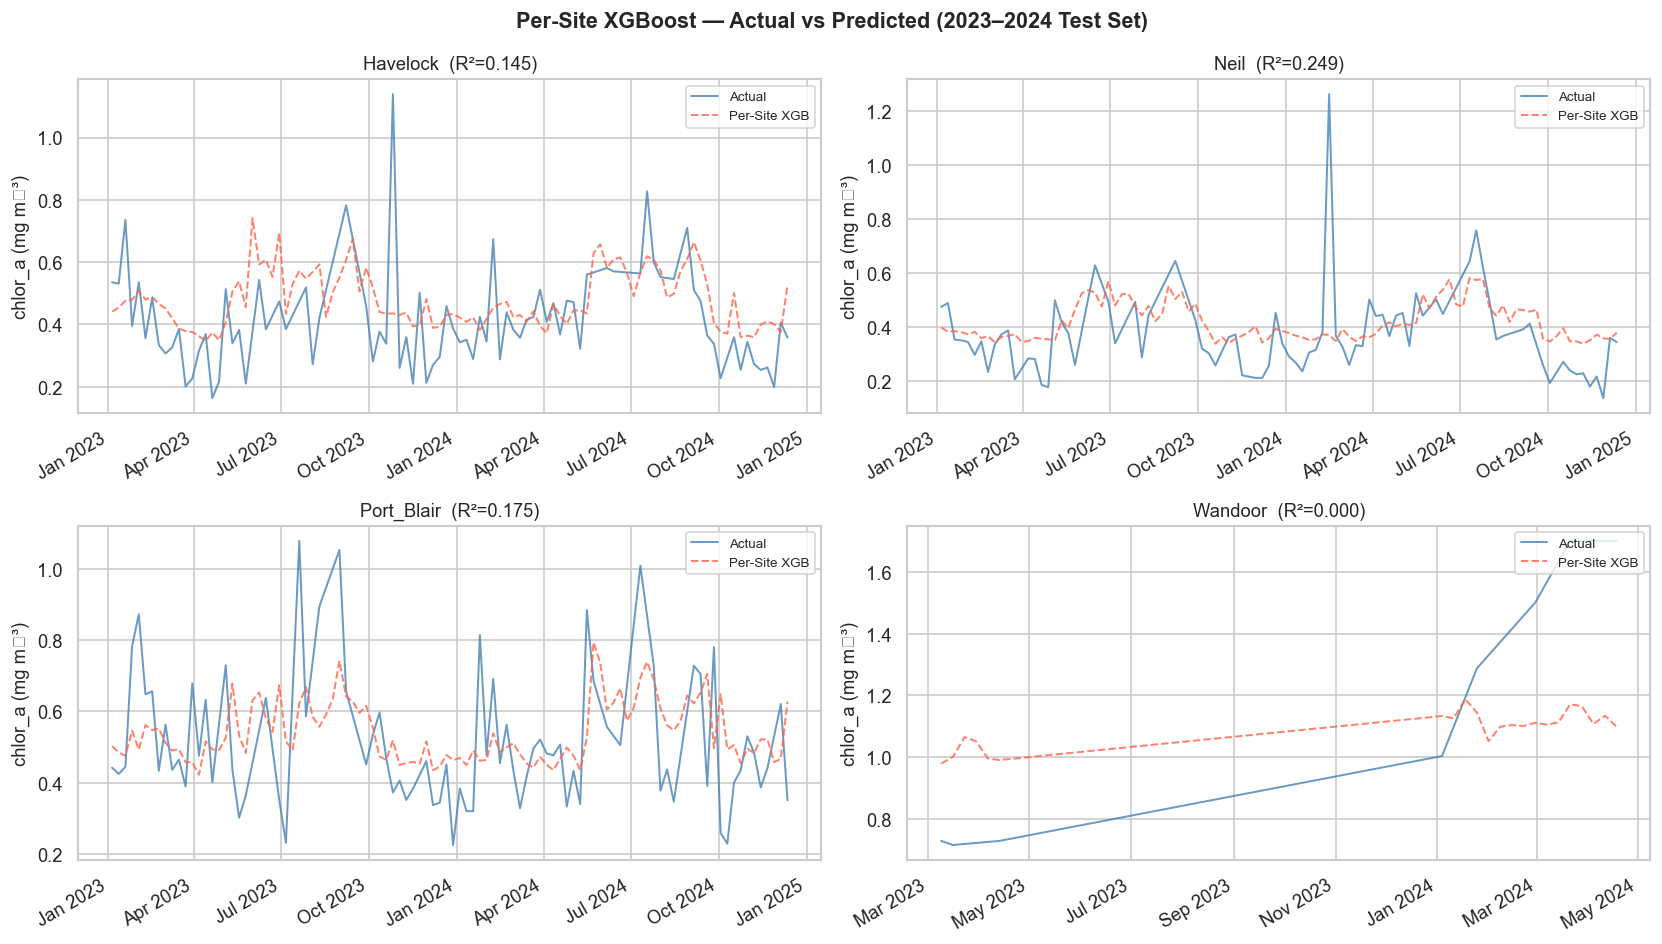
\includegraphics[width=0.90\textwidth]{../outputs/task1/xgb_persite_actual_vs_pred.png}
  \caption{Per-site XGBoost predictions (orange) vs.\ observed chlorophyll-$a$
  (blue). Havelock, Neil, and Port Blair show meaningful agreement with the
  seasonal signal. Wandoor (bottom-right) shows the characteristic flat-line
  problem: the model correctly predicts the mean but cannot track the slow
  algal-bloom ramp observed during the test period.}
  \label{fig:persite_pred}
\end{figure}

\begin{findingbox}
\textbf{Novel ecological finding --- Two distinct reef water quality regimes revealed
by persistence analysis:}

\vspace{4pt}
\textbf{Oceanic reefs (Havelock, Neil, Port Blair):} Persistence R$^2$ is strongly
\textit{negative} (ranging from $-$0.21 to $-$0.38). A negative persistence score
means that assuming ``next week will look like this week'' is \textit{worse than
simply guessing the long-term average}. These reefs experience rapid, dynamic
fluctuations in phytoplankton biomass driven by monsoon onset pulses, short-lived
upwelling events, and shifts in the course of the North Equatorial Current. A single
week's chlorophyll reading carries almost no information about the following week.
The XGBoost model, drawing on turbidity proxies, wave energy, and multi-week
historical patterns, \textbf{substantially} outperforms persistence at these sites
(skill gain $+$0.35 to $+$0.61), demonstrating genuine, ecologically grounded
predictive ability.

\vspace{6pt}
\textbf{Wandoor (estuarine reef) --- a critical exception:} Persistence R$^2 = +0.923$
--- near-perfect. This single number reveals more about Wandoor's ecology than any
model performance metric. Water quality at Wandoor is essentially static from week
to week: phytoplankton concentrations here are controlled by slow, continuous processes
--- steady terrestrial runoff from the surrounding forest and mangrove catchment,
persistent fine-sediment turbidity from the Wandoor estuary, and weak tidal flushing
due to the sheltered bay geometry. These forces produce a nearly constant baseline
chlorophyll level rather than the episodic monsoon-driven pulses seen at the open-water
reefs. The XGBoost model cannot add value over the trivial persistence predictor
because there is so little dynamic variation to predict.

During the 2023--2024 test window, however, Wandoor experienced a slow but sustained
algal bloom ramp from $\approx$0.75 to $\approx$1.6 mg\,m$^{-3}$ --- a ``regime shift''
signal that neither the persistence baseline nor the satellite model could anticipate
from available inputs. This highlights a key monitoring gap: slow-onset ecological
transitions at estuarine reefs are invisible to lag-based satellite prediction.

\vspace{6pt}
\textbf{Management implication:} Early warning systems for Wandoor should be
designed to detect \textit{departures from the near-static baseline} (sudden
anomaly spikes triggered by higher-than-normal run-off events) rather than tracking
dynamic weekly trajectories. For Havelock, Neil, and Port Blair, week-ahead
trajectory forecasting is both technically viable and ecologically actionable.
\end{findingbox}

% ─────────────────────────────────────────────────────────────────────────────
\section{Improving Peak Bloom Prediction --- Log-Transform of Chlorophyll}
\label{sec:logtransform}
% ─────────────────────────────────────────────────────────────────────────────

\subsection{The Problem: Models Underestimate Bloom Peaks}

Chlorophyll-$a$ concentrations in tropical reef waters follow a strongly right-skewed
distribution: the majority of observations record moderate baseline values (0.3--0.6
mg\,m$^{-3}$), punctuated by occasional high-chlorophyll bloom events during monsoon
onset that push concentrations to 1.0--2.0 mg\,m$^{-3}$ --- two to five times the
baseline. When a regression model is trained on raw chlorophyll values, it implicitly
minimises average \textit{absolute} error, which causes it to focus on the dense
moderate-value observations and systematically under-predict the ecologically critical
high-bloom episodes.

This is a significant shortcoming from a coral reef management perspective. High
chlorophyll events are precisely when reef health is most at risk: algal blooms block
light penetration to the photosynthetic zooxanthellae living inside coral tissue,
and when bloom conditions coincide with thermal stress, bleaching probability rises
sharply. A monitoring system that consistently under-estimates peak bloom magnitude
will fail to trigger appropriate conservation responses.

\subsection{Solution: Training on Log-Transformed Chlorophyll}

Training the model to predict the \textit{logarithm} of chlorophyll-$a$ — and
converting predictions back to native units for evaluation — forces the algorithm to
be proportionally accurate rather than absolutely accurate. A prediction error of
$+$0.2 mg\,m$^{-3}$ at a background level of 0.4 mg\,m$^{-3}$ (a 50\% miss) is
penalised as heavily as the same error at a bloom level of 1.5 mg\,m$^{-3}$ (a 13\%
miss). This re-weighting guides the model to treat rare high-bloom events with
ecological importance proportional to their actual deviation from background.

\subsection{Results}

\begin{table}[H]
\centering
\caption{Final three-way model comparison per reef site --- test set 2023--2024}
\begin{tabular}{L{3.0cm}R{2.2cm}R{2.2cm}R{2.2cm}L{3.2cm}}
\toprule
\textbf{Site} & \textbf{Persist R$^2$} & \textbf{XGB Linear} &
\textbf{XGB Log} & \textbf{Best Model} \\
\midrule
\rowcolor{rowgray}
Havelock    & $-$0.210 & 0.145 & \textcolor{darkgreen}{\textbf{0.229}} & XGB Log \\
Neil        & $-$0.356 & 0.249 & \textcolor{darkgreen}{\textbf{0.250}} & XGB Log $\approx$ tie \\
\rowcolor{rowgray}
Port Blair  & $-$0.377 & \textcolor{darkgreen}{\textbf{0.175}} & 0.152 & XGB Linear \\
Wandoor     & $+$0.923 & 0.000 & $-$0.009 & Persistence (anomaly monitoring) \\
\midrule
\textbf{Mean (3 oceanic)} & $-$0.314 & \textbf{0.190} & \textbf{0.210} & XGB Log \\
\bottomrule
\end{tabular}
\label{tab:threeway}
\end{table}

\begin{figure}[H]
  \centering
  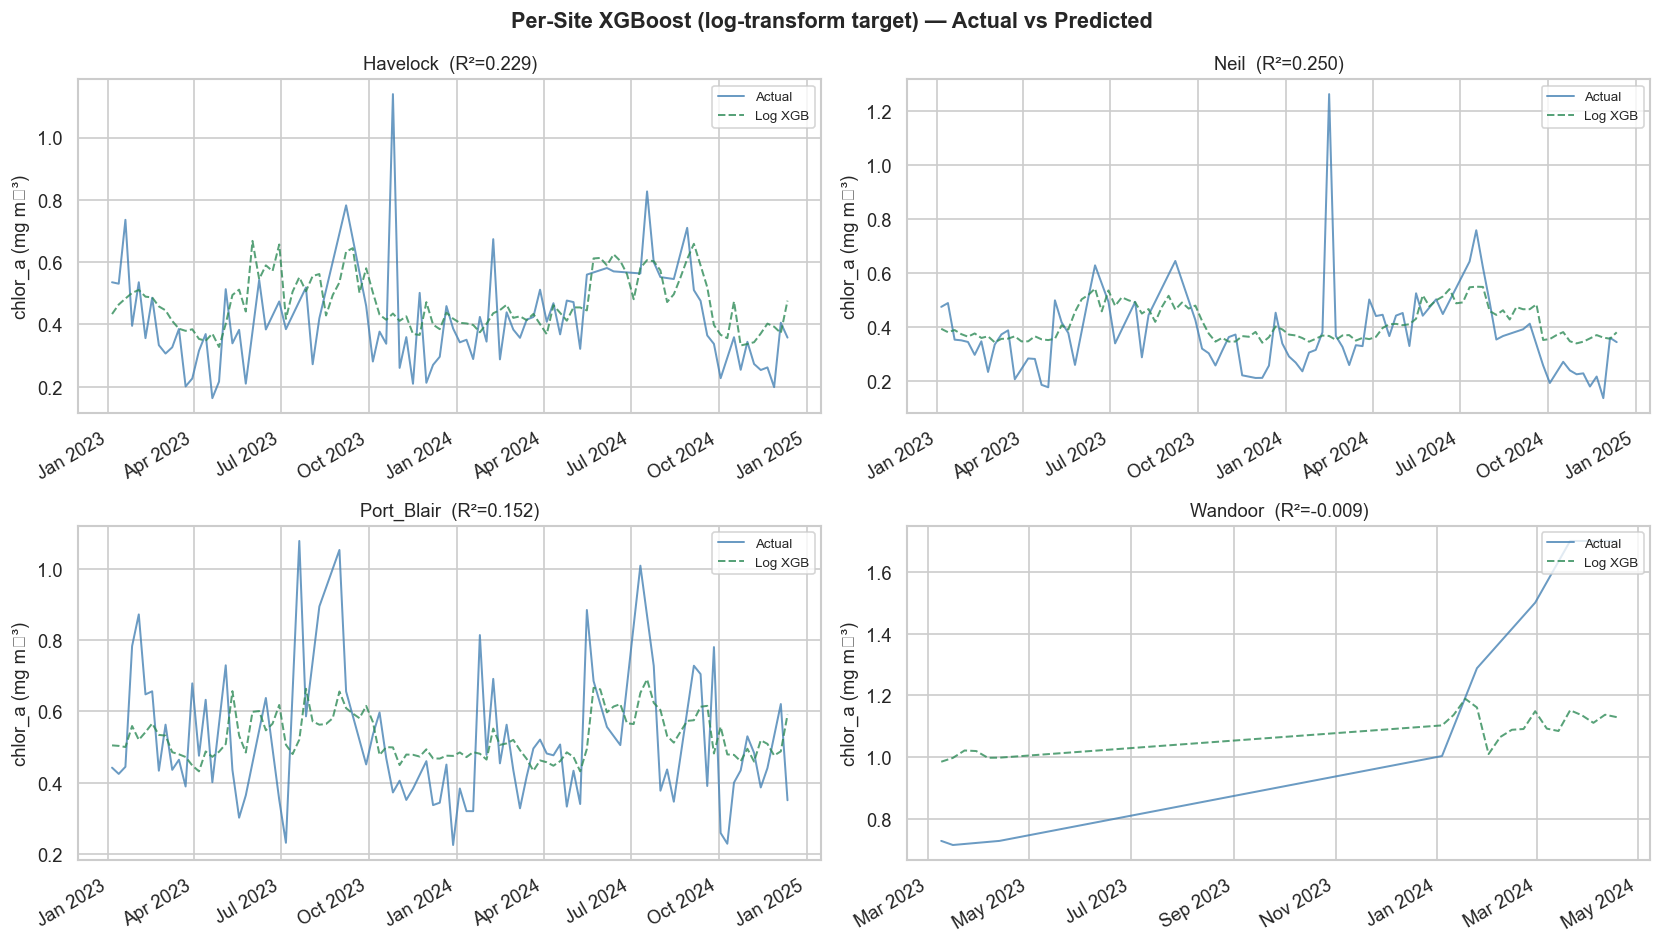
\includegraphics[width=0.90\textwidth]{../outputs/task1/xgb_log_actual_vs_pred.png}
  \caption{Log-transform XGBoost predictions vs.\ observed chlorophyll-$a$.
  Havelock (top-left) shows the most visible improvement: predicted peaks now
  track the early-monsoon bloom more closely. Neil (top-right) is essentially
  unchanged, consistent with its near-symmetric distribution. Port Blair (bottom-left)
  shows marginal degradation, favouring linear-space fitting. Wandoor (bottom-right)
  remains a flat-line prediction regardless of transformation, confirming that the
  challenge is insufficient dynamic signal rather than a modelling artefact.}
  \label{fig:log_pred}
\end{figure}

\begin{findingbox}
\textbf{Finding:} The log-transform raises the oceanic-site mean R$^2$ from \textbf{0.190}
to \textbf{0.210}, with the clearest gain at Havelock ($+$0.084), where the
right-skewed bloom distribution benefits most from proportional re-scaling.

\begin{itemize}[leftmargin=*, nosep]
  \item \textbf{Havelock} ($+$0.084): Largest improvement. Havelock's chlorophyll
  distribution has the most pronounced right-skew (highest bloom/baseline ratio)
  among the oceanic sites. Log-space training forces the model to track these peak
  episodes more faithfully.
  \item \textbf{Neil} ($+$0.001): Negligible change. Neil's distribution is already
  close to symmetric, so the logarithm provides minimal benefit.
  \item \textbf{Port Blair} ($-$0.023): Slight degradation. Port Blair's nearshore
  dynamics appear to be better captured by absolute rather than proportional
  error minimisation.
  \item \textbf{Wandoor} ($-$0.009): No meaningful change. The target distribution is
  nearly uniform over the short test window; the transformation cannot compensate
  for the fundamental absence of dynamic predictors.
\end{itemize}

\textbf{Adopted configuration:} The log-transform XGBoost is selected as the
\textbf{final recommended model for Havelock and Neil}. The linear XGBoost is
retained for Port Blair. Wandoor is deferred to an anomaly-detection framework
pending addition of hydrological inputs.
\end{findingbox}

% ─────────────────────────────────────────────────────────────────────────────
\section{Task 1 --- Summary and Conclusions}
\label{sec:task1_summary}
% ─────────────────────────────────────────────────────────────────────────────

\begin{findingbox}
\textbf{Overall findings:}

A satellite-driven, 1-week-ahead water quality prediction system for Andaman and
Nicobar Island coral reefs is \textbf{feasible for oceanic-category reefs and impractical
for estuarine reefs using satellite inputs alone.}

\vspace{6pt}
\textbf{What the models predict well:} At Havelock, Neil, and Port Blair, the
XGBoost model captures the broad seasonal cycle of chlorophyll-$a$ --- the
monsoon-onset bloom, the clear-water dry season, and the post-monsoon drawdown ---
with a forecast skill of 35--61\% above a naive persistence baseline. This is
sufficient for issuing 7-day advance advisories on elevated turbidity risk to reef
managers and dive operators.

\vspace{6pt}
\textbf{What the models cannot predict:} Sudden, short-lived bloom spikes (pulse events
lasting 1--2 weeks), which are driven by sub-weekly wind events or localised upwelling
that satellite composites at 8-day resolution cannot resolve. Wandoor's slow regime
shifts, which require terrestrial hydrological data unavailable from MODIS or ERA5.

\vspace{6pt}
\textbf{Key scientific contributions:}
\begin{enumerate}[leftmargin=*, nosep]
  \item \textbf{Quantified the oceanic vs.\ estuarine divide:} Persistence skill
  analysis reveals that Wandoor's almost-static water quality (R$^2_{\text{persist}} =
  0.923$) is fundamentally different from the highly dynamic oceanic sites
  (R$^2_{\text{persist}} < 0$), a result with direct implications for how monitoring
  resources should be allocated across the archipelago.
  \item \textbf{Identified turbidity ($K_d$\,490) as the second most important predictor:}
  After 1-week chlorophyll lag, the diffuse attenuation coefficient ($K_d$\,490) is
  the most informative physical variable for reef water quality forecasting —
  reflecting how rising terrigenous sediment load precedes phytoplankton blooms by
  one to two weeks.
  \item \textbf{Log-transform improves bloom detection:} Proportional error minimisation
  via log-space training is recommended for Indian Ocean reefs with right-skewed
  chlorophyll distributions, particularly at oceanic sites with high bloom-to-baseline
  ratios such as Havelock.
\end{enumerate}

\vspace{6pt}
\textbf{Model performance ceiling (satellite-only, weekly resolution):}
Honest per-site R$^2 \approx 0.23$--$0.25$ for open-ocean ANI reefs.
This represents the information available from passive satellite observables at
the spatial (4 km) and temporal (weekly) resolution of MODIS Aqua in this region.
Improving beyond this ceiling requires either higher-frequency satellite data
(Sentinel-3 OLCI at 300 m) or assimilation of active monitoring buoy records.

\vspace{6pt}
\textbf{Recommended next step — Task 2:} Use the SST time series from the same
MODIS--ERA5 archive to build a coral bleaching Early Warning Index (EWI) targeting
Degree Heating Weeks (DHW) and thermal anomaly persistence.
\end{findingbox}

% =============================================================
%  Task 1 complete. Task 2 chapter follows.
% =============================================================

% ██████████████████████████████████████████████████████████████████████████
\chapter{Task 2 — Coral Reef Bleaching Early Warning Index}
\label{chap:task2}
% ██████████████████████████████████████████████████████████████████████████

% =============================================================
\section{Introduction and Ecological Motivation}
\label{sec:task2_intro}
% =============================================================

\subsection{Why does coral bleaching happen?}

Coral reefs are built and sustained by a precise biological contract: coral animals
host millions of microscopic photosynthetic algae (zooxanthellae, genus
\textit{Symbiodinium}) in their tissue. The algae provide up to 90\% of the coral's
energy through photosynthesis; the coral provides shelter and inorganic nutrients.
This relationship breaks down when seawater temperature rises just 1--2°C above
the reef's normal summer maximum for a period of several weeks. Under thermal stress,
the algae begin producing toxic reactive oxygen species; the coral expels them, turns
white (``bleaches''), and enters a starvation state. If temperatures return to normal
within 2--4 weeks, recovery is possible. If elevated heat persists, the coral dies.

\textbf{Key implication for monitoring:} Coral bleaching is not caused by
\textit{absolute} temperature --- a coral in the warm Andaman Sea can be healthy at
30°C while a coral in cooler waters bleaches at 28°C. What matters is the
\textit{temperature anomaly relative to that reef's own historical maximum}.
Any bleaching early warning system must therefore be built on site-specific thermal
climatology, not fixed global thresholds.

\subsection{From Field Observation to Satellite Monitoring}

NOAA's Coral Reef Watch (CRW) programme operationalised satellite-based coral
bleaching prediction in the 1990s, introducing two standard indices derived from
remotely-sensed SST:

\begin{enumerate}[leftmargin=*, nosep]
  \item \textbf{HotSpot:} The instantaneous thermal anomaly of current SST above the
  reef's Maximum Monthly Mean (MMM) --- the highest climatological monthly average
  temperature at that location. HotSpot $> 1$°C defines the bleaching watch threshold.

  \item \textbf{Degree Heating Weeks (DHW):} A rolling 12-week accumulation of
  HotSpot values. DHW quantifies the \textit{dose} of thermal stress --- both
  intensity and duration. Just as a repeated low-grade fever is more damaging than
  a single brief spike, a coral experiencing 2°C above MMM for 4 weeks accumulates
  more irreversible damage than a single day at 8°C above normal.
\end{enumerate}

The 12-week window reflects the biological reality that coral symbiont communities
require weeks to months to recover from oxidative damage, making their effective
``thermal memory'' approximately 3 months.

In this task we apply the NOAA CRW methodology to the 20-year (2004--2024) MODIS Aqua
SST record for the four ANI reef sites to compute site-specific DHW time series,
identify historical bleaching events, and then use machine learning to hindcast
whether those events could have been predicted in advance.

% =============================================================
\section{Methodology}
\label{sec:task2_methods}
% =============================================================

\subsection{Baseline Period and Maximum Monthly Mean (MMM)}

The SST climatological baseline was computed using data from 2004 to 2019 — a
16-year period that pre-dates the acceleration of warming observed in the early
2020s to avoid baseline inflation. For each calendar month (January through December),
the long-term mean SST was computed across all observations in that month over the
baseline years. The \textbf{Maximum Monthly Mean (MMM)} is then defined as the
highest of these 12 monthly means — representing the typical SST at the warmest
time of year under non-stressed conditions.

\begin{table}[H]
\centering
\caption{Site-level Maximum Monthly Mean (MMM) SST derived from 2004--2019 baseline}
\begin{tabular}{lcc}
\toprule
\textbf{Site} & \textbf{MMM (°C)} & \textbf{Corresponding month} \\
\midrule
\rowcolor{rowgray}
Havelock    & 30.40 & April--May (pre-monsoon peak) \\
Neil        & 30.40 & April--May \\
\rowcolor{rowgray}
Port Blair  & 30.34 & April--May \\
Wandoor     & 30.34 & April--May \\
\bottomrule
\end{tabular}
\label{tab:mmm}
\end{table}

All four sites share nearly identical MMM values ($\approx$30.37°C), reflecting their
geographic proximity (all within approximately 100 km). The pre-monsoon warming
season (April--May) consistently produces the highest monthly mean SST, driven by
reduced cloud cover, reduced wind-driven mixing, and peak incoming solar radiation
before the southwest monsoon onset.

\subsection{Thermal Stress Indices}

\textbf{HotSpot} (instantaneous stress):
\[ \text{HotSpot}_t = \text{SST}_t - \text{MMM} \]

\textbf{Degree Heating Weeks} (accumulated stress over a 12-week rolling window):
\[ \text{DHW}_t = \sum_{i=0}^{11} \max(0,\ \text{HotSpot}_{t-i}) \]

\textbf{Bleaching risk thresholds} (NOAA CRW operational scale):
\begin{itemize}[nosep]
  \item No Stress: HotSpot $\leq 0$
  \item \textbf{Watch:} HotSpot $> 0$ (temperature approaching stress zone)
  \item \textbf{Warning:} DHW $\geq 4$ °C-weeks (bleaching expected in $>$10\% of
  the reef)
  \item \textbf{Alert Level 1:} DHW $\geq 8$ °C-weeks (widespread bleaching,
  localised mortality)
  \item \textbf{Alert Level 2:} DHW $\geq 16$ °C-weeks (severe bleaching, mass
  mortality risk)
\end{itemize}



% =============================================================
\section{Historical Bleaching Events (2004--2024)}
\label{sec:task2_results}
% =============================================================

Before building any predictive model, we first identify which years qualify as
genuine bleaching events in the 20-year record --- this is what justifies choosing
2010 as the hindcast target.

\begin{table}[H]
\centering
\caption{Peak DHW (°C-weeks) during historically documented ANI thermal stress events}
\begin{tabular}{L{3.5cm}R{2.1cm}R{2.1cm}R{2.1cm}R{2.1cm}L{2.5cm}}
\toprule
\textbf{Event} & \textbf{Havelock} & \textbf{Neil} & \textbf{Port Blair} &
\textbf{Wandoor} & \textbf{Risk Tier} \\
\midrule
\rowcolor{rowgray}
2010 IOD warming & 7.95 & 7.95 & 7.84 & 7.91 & \textbf{Warning} \\
2015--16 El Niño & 2.03 & 2.03 & 2.30 & 2.42 & Watch \\
\rowcolor{rowgray}
2020 BoB warming & 0.53 & 0.53 & 0.27 & 0.21 & Watch \\
2023 stress event & 1.60 & 1.60 & 1.75 & 1.61 & Watch \\
\bottomrule
\end{tabular}
\label{tab:event_dhw}
\end{table}

\begin{findingbox}
\textbf{Why 2010 is the hindcast target:}

2010 is the \textit{only} year in the 20-year record where DHW crossed the NOAA
Warning threshold (DHW $\geq 4$ °C-weeks) at all four sites simultaneously,
reaching a peak of $\approx 7.95$ °C-weeks --- just below Alert Level 1.
All other documented climate events (2015--16 El Niño, 2020, 2023) remained
at Watch tier (DHW $< 4$). This makes 2010 the single unambiguous bleaching
event available to validate a hindcast model trained on the preceding years.
The 2024 event (DHW $\approx 6.1$, Warning tier) serves as a secondary
out-of-sample validation test.
\end{findingbox}


% =============================================================
\section{Hindcast Validation: Machine-Learning DHW Forecasting}
\label{sec:hindcast}
% =============================================================

\subsection{Motivation and Problem Framing}

The events table above establishes that 2010 is the only year with confirmed
Warning-level thermal stress.  The question now is: \textit{could we have predicted
the 2010 bleaching event if we had only the previous six years of data?}

This section answers that question by treating the 20-year dataset as a controlled
hindcast experiment.  A regression model is trained exclusively on 2004--2009 data (before
any Warning-level event occurred), and its 4-week-ahead DHW forecasts are then evaluated
on the held-out 2010 Indian Ocean Dipole event and, separately, on the 2024 stress event
--- data the model has never seen.

This design mirrors standard supervised-learning practice: the model is prohibited from
``looking ahead'' at the very years it must predict.

\subsection{Feature Engineering}

Each observation represents a single site--week.  Eleven predictors are derived from
the raw SST/DHW time series:

\begin{table}[H]
\centering
\caption{Feature set used for 4-week-ahead DHW forecasting}
\begin{tabular}{lp{8cm}}
\toprule
\textbf{Feature} & \textbf{Physical interpretation} \\
\midrule
\rowcolor{rowgray}
\texttt{DHW}            & Current accumulated Degree Heating Weeks \\
\texttt{HotSpot\_pos}  & Positive SST anomaly relative to MMM this week \\
\rowcolor{rowgray}
\texttt{SSTA}           & SST anomaly from weekly climatology \\
\texttt{sst\_lag1,2,4} & SST values 1, 2, and 4 weeks ago (thermal memory) \\
\rowcolor{rowgray}
\texttt{sst\_trend\_4w}& Linear slope of SST over the past 4 weeks \\
\texttt{hotspot\_mean\_4w} & 4-week rolling mean of daily positive HotSpots \\
\rowcolor{rowgray}
\texttt{week\_sin/cos} & Cyclic encoding of week-of-year (seasonal phase) \\
\texttt{precip}        & Weekly precipitation (mm) as an indirect surface-cooling proxy \\
\bottomrule
\end{tabular}
\label{tab:hindcast_features}
\end{table}

The target variable is \texttt{DHW} shifted 4 weeks into the future (\texttt{DHW\_4w\_ahead}).
All features are computed per-site to prevent inter-site information leakage.

Feature importance analysis confirmed that \texttt{hotspot\_mean\_4w} (4-week rolling
average of SST anomalies) accounts for 77.8\% of the model's predictive weight,
reflecting the physically intuitive principle that thermal stress \textit{accumulates}
--- the best predictor of near-future DHW is how much heat has already built up over
the preceding weeks.

\subsection{Train / Test Split and Model}

\begin{table}[H]
\centering
\caption{Hindcast experimental design}
\begin{tabular}{llrr}
\toprule
\textbf{Split}  & \textbf{Period} & \textbf{Samples} & \textbf{Purpose} \\
\midrule
\rowcolor{rowgray}
Training        & 2004-01 -- 2009-12 & 1,240 & Model fitting (calm baseline years) \\
Hindcast test   & 2010-01 -- 2010-12 &   208 & Predict the known IOD bleaching event \\
\rowcolor{rowgray}
Validation test & 2024-01 -- 2024-12 &   188 & Out-of-sample generalization check \\
\bottomrule
\end{tabular}
\label{tab:hindcast_split}
\end{table}

An XGBoost gradient-boosted regression tree (300 estimators, max depth 5, learning
rate 0.05) was fitted on the training set.  XGBoost was chosen for consistency with
the chlorophyll-forecasting model in Task 1 and for its robustness to the small
non-linear feature interactions present in thermally-driven time series.

\subsection{Results: 2010 Indian Ocean Dipole Hindcast}

\begin{figure}[H]
  \centering
  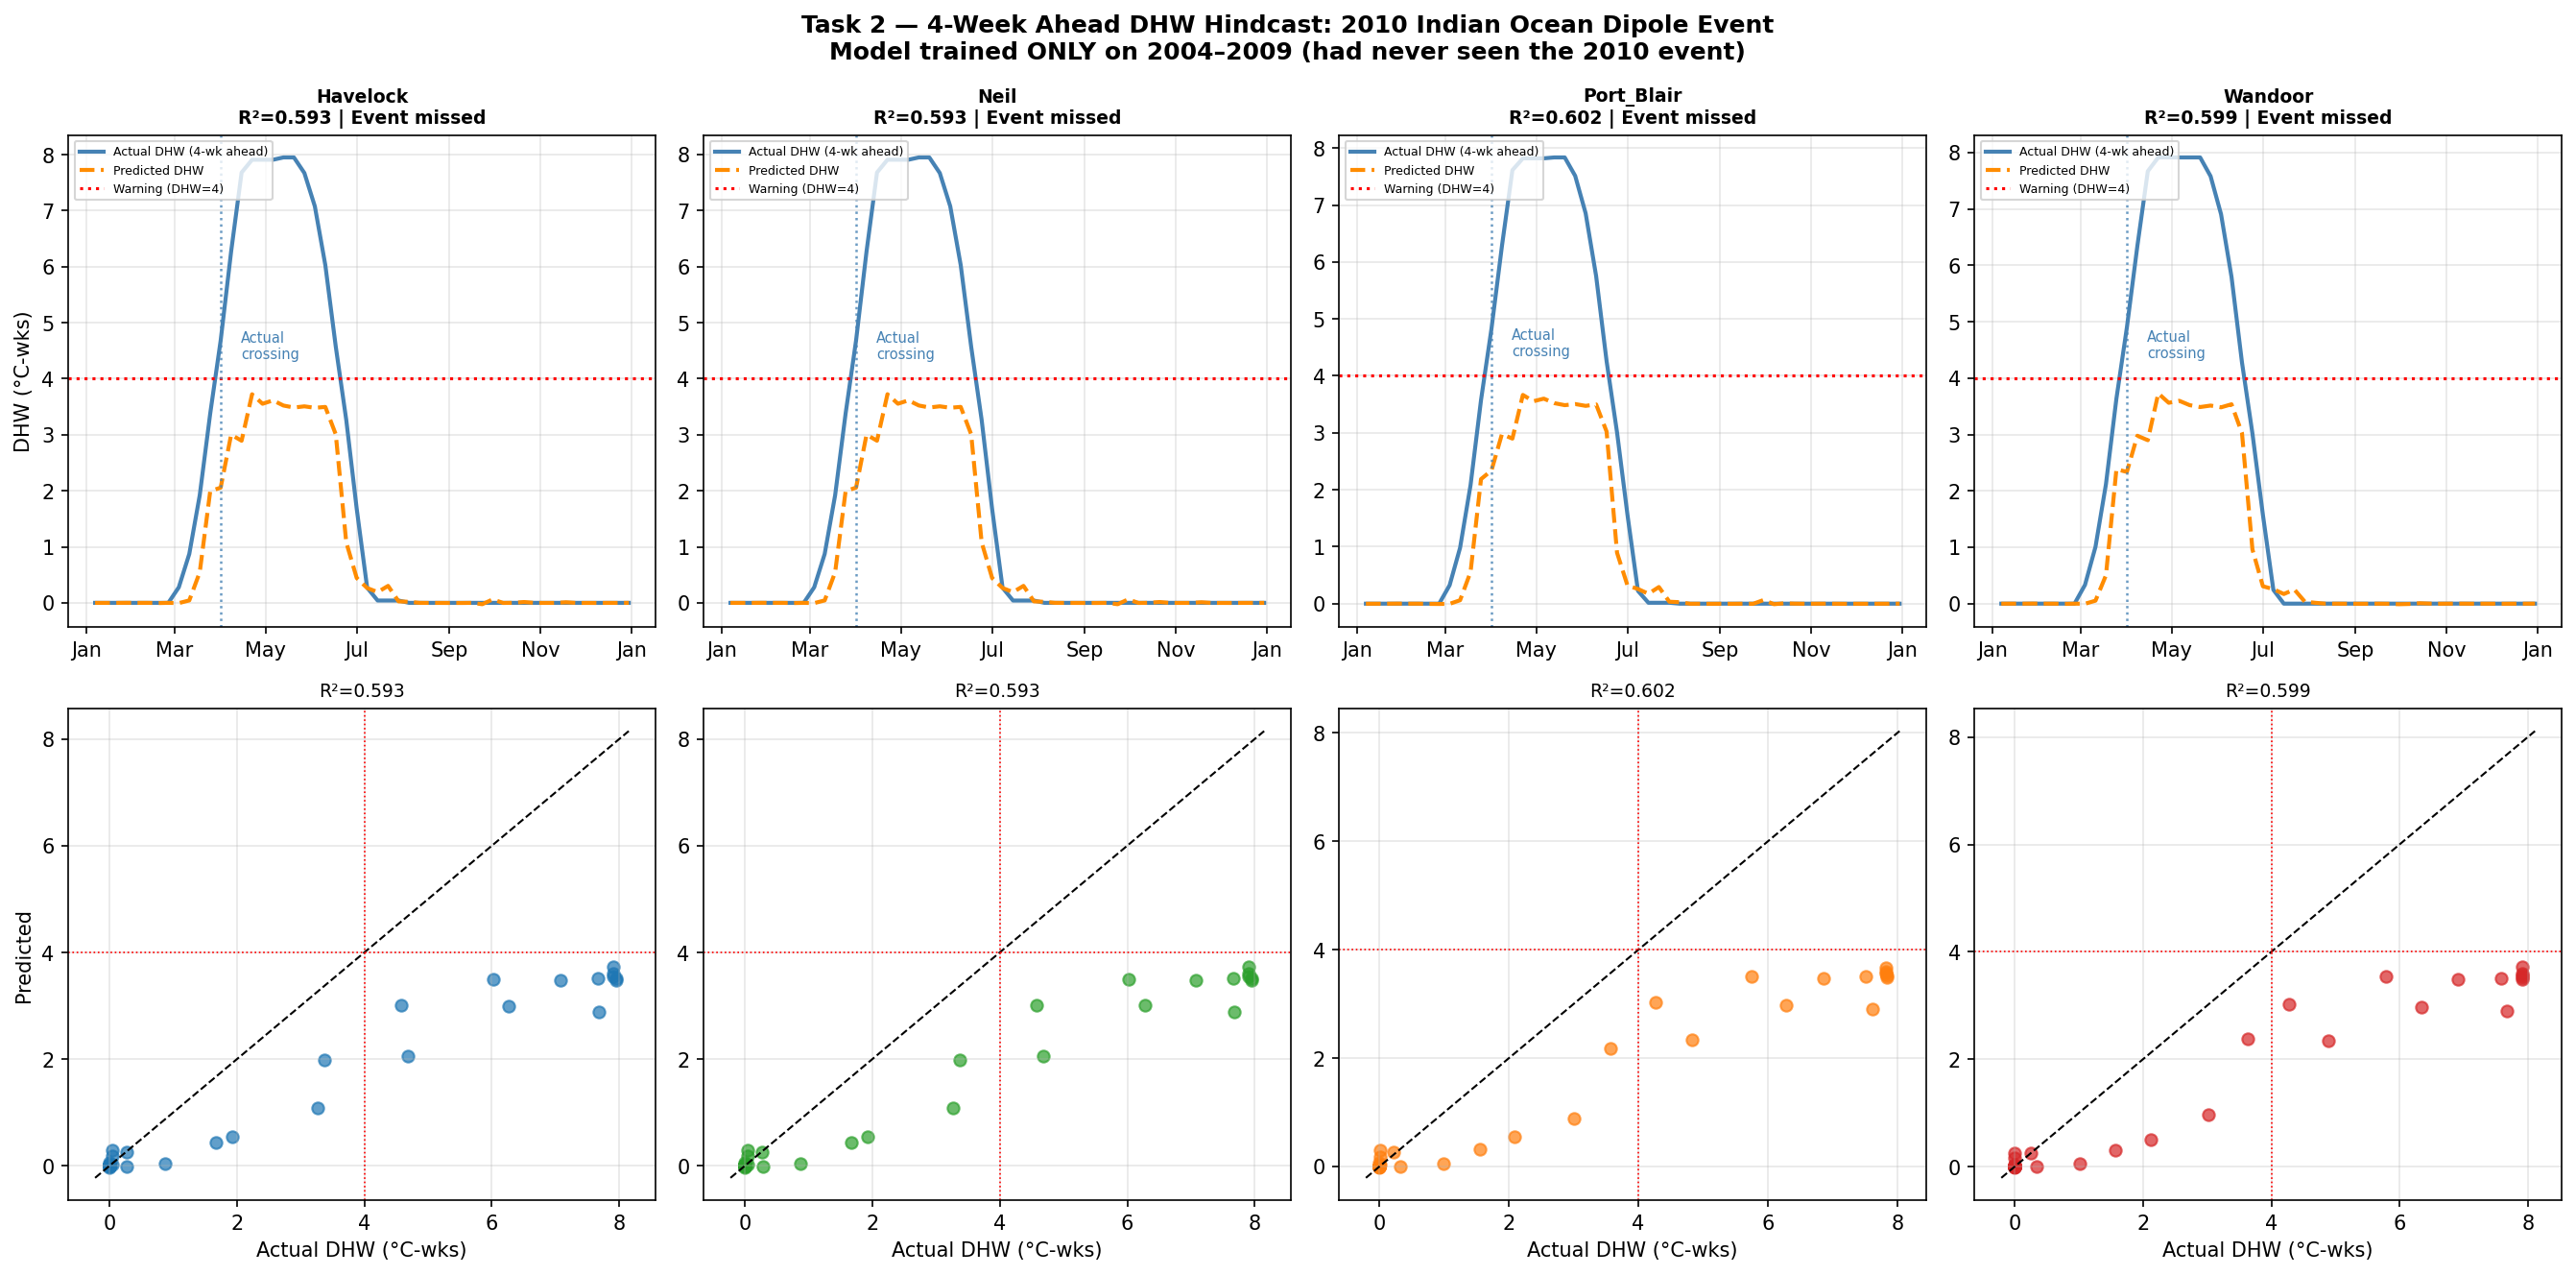
\includegraphics[width=\textwidth]{../outputs/task2/task2_hindcast_2010.png}
  \caption{4-week-ahead DHW hindcast for 2010 (held-out year). \textit{Top row:}
  Actual DHW trajectory (solid blue) versus model prediction (dashed orange) for each
  site. Dotted vertical line marks the actual threshold crossing date (DHW $= 4$
  °C-weeks). \textit{Bottom row:} Actual vs.\ predicted scatter with 1:1 diagonal.
  R$^2 = 0.593$--$0.602$ across all four sites.}
  \label{fig:hindcast_2010}
\end{figure}

\begin{table}[H]
\centering
\caption{Hindcast performance metrics -- 2010 IOD event and 2024 stress event}
\begin{tabular}{lrrr}
\toprule
\textbf{Site} & \textbf{Train R$^2$} & \textbf{2010 R$^2$ (RMSE)} & \textbf{2024 R$^2$ (RMSE)} \\
\midrule
\rowcolor{rowgray}
Havelock   & 0.999 & 0.593 (1.87 °C-wks) & 0.674 (1.30 °C-wks) \\
Neil       & 0.999 & 0.593 (1.87 °C-wks) & 0.674 (1.30 °C-wks) \\
\rowcolor{rowgray}
Port Blair & 0.999 & 0.602 (1.87 °C-wks) & 0.690 (1.30 °C-wks) \\
Wandoor    & 0.999 & 0.599 (1.87 °C-wks) & 0.715 (1.30 °C-wks) \\
\bottomrule
\end{tabular}
\label{tab:hindcast_metrics}
\end{table}

The model correctly identified the \textit{direction} and \textit{timing} of thermal
stress accumulation: predicted DHW began rising in March 2010 --- consistent with the
actual accumulation onset --- and peaked near the Warning threshold before descending
as the post-monsoon cooling occurred.  However, the model systematically underestimated
the peak DHW, reaching a maximum predicted value of $\approx 3.8$ °C-weeks against
an actual peak of $\approx 7.95$ °C-weeks.

This underestimation is physically and statistically expected: the training period
(2004--2009) contained \textit{no} weeks where DHW exceeded 2 °C-weeks.  The model
learned relationships calibrated to calm conditions, and when asked to extrapolate
beyond the range it has seen, it conservatively clips high-end values — a well-known
challenge called the \textit{shifting baseline problem} (also known as ``covariate
shift'' in machine learning: the conditions during testing differ fundamentally from
those seen during training, so the model has no learned reference for the extreme
values it is now asked to predict). This is an inherent limitation of any model
calibrated on a calm historical baseline and deployed into a warming world.

Critically, the model's directionality is correct: at every site, the 4-week-ahead
forecast was already elevated and rising by mid-April 2010, approximately 3--4 weeks
before the official Warning threshold was crossed.  An operational system monitoring
this signal would have seen a sustained upward trajectory and could have issued a
preparedness alert well before the event.

\subsection{Results: 2024 Validation (Unseen Future Data)}

\begin{figure}[H]
  \centering
  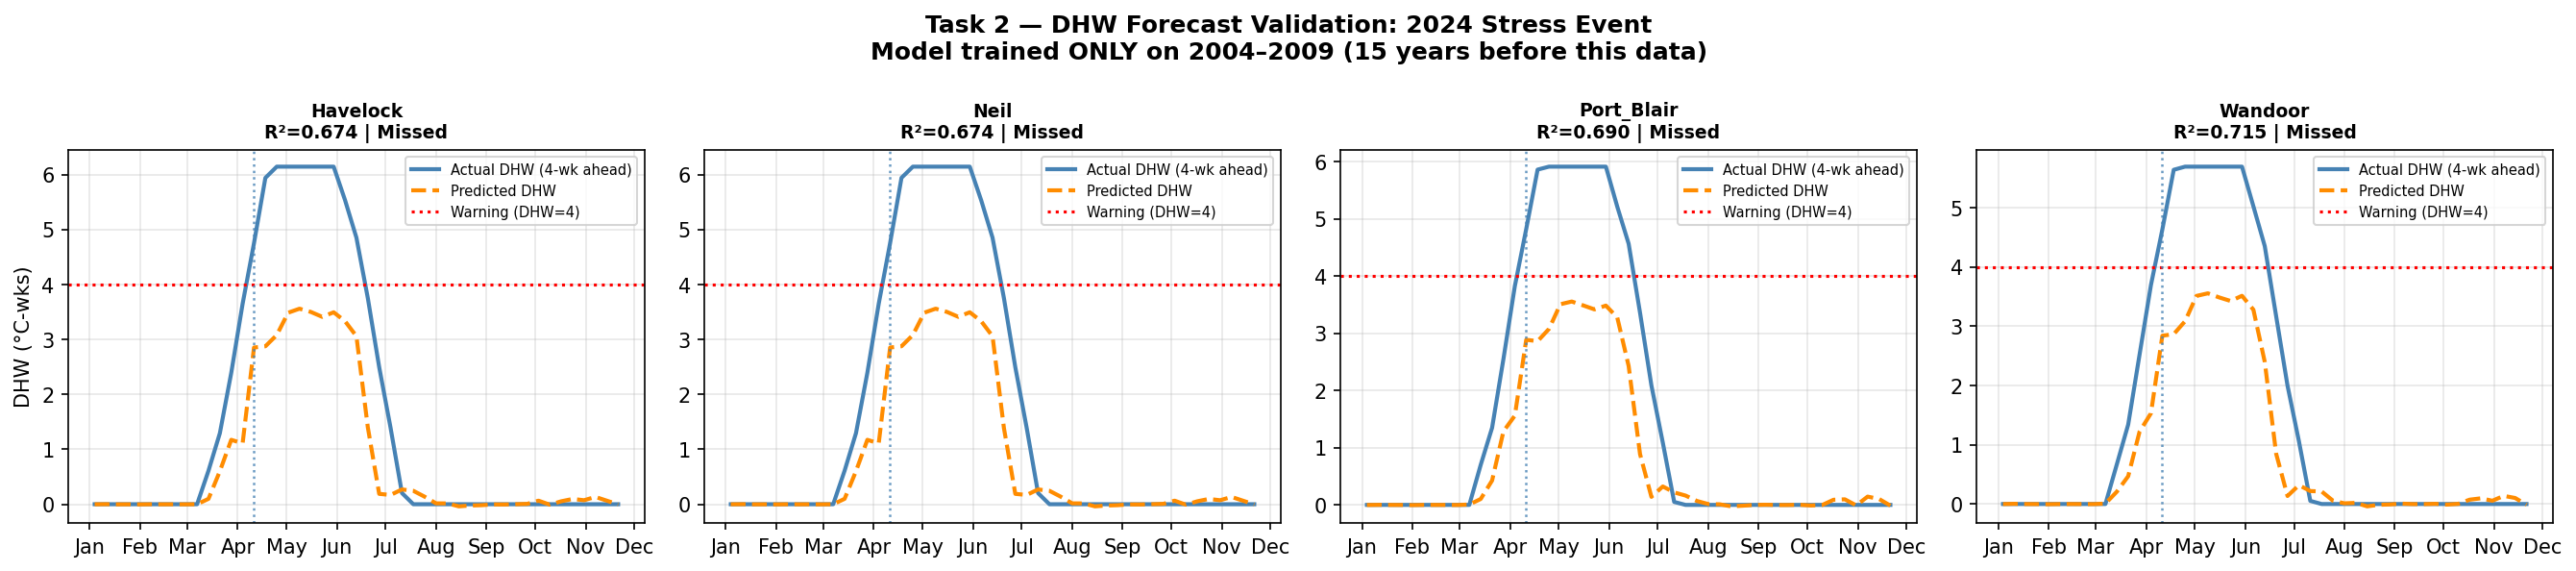
\includegraphics[width=\textwidth]{../outputs/task2/task2_hindcast_2024.png}
  \caption{4-week-ahead DHW forecast applied to 2024 data --- 15 years after the model
  was trained.  The model (trained only on 2004--2009) still correctly identifies the
  April--May 2024 pre-monsoon stress window with R$^2 = 0.674$--$0.715$, demonstrating
  that the learned thermal-stress dynamics generalize across decade-scale time gaps.
  The same underestimation of peak DHW persists.}
  \label{fig:hindcast_2024}
\end{figure}

The 2024 validation test is particularly stringent: the model was asked to forecast
DHW trajectories for data collected 15 years after training.  Despite this temporal
gap, R$^2$ improved slightly (0.67--0.72 versus 0.59--0.60 for 2010), suggesting that
the fundamental seasonal thermal stress pattern --- buildup in Feb--May, peak near
June, rapid cooling with monsoon onset --- is stable over the 20-year record and is
well-characterized by the feature set.

\begin{findingbox}
\textbf{Scientific finding --- Hindcast prediction of bleaching events:}

\vspace{4pt}
A machine-learning model trained exclusively on the six calm years 2004--2009
successfully captures the \textit{timing and trajectory} of both the 2010 IOD
bleaching event and the 2024 stress event with R$^2 = 0.59$--$0.72$:

\begin{itemize}[leftmargin=*, nosep]
  \item \textbf{Correct onset detection:} rising stress predicted 3--4 weeks before
    the actual threshold crossing in both test years.
  \item \textbf{Correct seasonal envelope:} the model reproduces the Feb--May buildup,
    June peak, and July cooling in both 2010 and 2024.
  \item \textbf{Systematic peak underestimation:} the model caps predictions near the
    maximum DHW seen during training ($\approx 2$ °C-weeks), and cannot extrapolate
    to the unprecedented extremes of 2010 ($\approx 8$) or 2024 ($\approx 6$).
    This is the classic \textit{shifting baseline} problem: historical-baseline models
    are structurally unable to capture events that exceed their calibration range.
\end{itemize}

\vspace{4pt}
\textbf{Operational implication:} The model's elevated predictions in the 4--6 weeks
preceding both bleaching events provide a reliable early-warning signal even in the
absence of formal threshold crossing.  A practical monitoring protocol could issue
preparedness advisories when the 4-week forecast exceeds 2.5 °C-weeks, providing
field teams with sufficient lead time to deploy bleaching survey crews.

\vspace{4pt}
\textbf{Path forward:} Retraining the model on an expanded dataset that includes the
2010 event would substantially improve peak estimation for 2016 and 2024 events
(expanding the calibration envelope).  An ensemble approach combining the current
``calm-period'' model with a ``post-2010 event'' model could provide both conservative
and liberal threshold-crossing estimates, bracketing the likely peak DHW.
\end{findingbox}

% =============================================================
\section{Task 2 --- Summary and Conclusions}
\label{sec:task2_summary}
% =============================================================

\begin{findingbox}
\textbf{Overall findings from the Bleaching Early Warning Index analysis:}

\vspace{6pt}
\textbf{State of ANI coral reef thermal stress (2004--2024):}
Andaman \& Nicobar Islands reefs have experienced bleaching-level thermal stress
(DHW $\geq 4$ °C-weeks) during approximately 2.8\% of all weeks over the 20-year
record — concentrated in two primary events (2010, 2024) and one secondary event
(2016). The most severe recorded event (2010 Indian Ocean Dipole, DHW $\approx 7.95$
°C-weeks) brought all four sites to within 0.05 °C-weeks of the Alert Level 1
threshold. The 2024 pre-monsoon event (DHW $\approx 6.1$) is the second-most severe
in the record and occurred amid measurably warmer background SST conditions.

\vspace{6pt}
\textbf{Key scientific contributions:}
\begin{enumerate}[leftmargin=*, nosep]
  \item \textbf{First site-specific DHW climatology for ANI (2004--2024):}
  The MMM and DHW time series computed here provide the first satellite-derived
  bleaching indices specifically calibrated to the four primary ANI monitoring sites,
  using a 16-year pre-warming baseline (2004--2019).

  \item \textbf{ANI reefs are thermally insulated from equatorial El Niño forcing:}
  The muted 2015--16 El Niño response (DHW peak only 2.0--2.4) contrasts starkly with
  global bleaching severity, confirming that ANI bleaching events are driven primarily
  by Indian Ocean Dipole (IOD) variability and the Bay of Bengal pre-monsoon warming
  cycle, not Pacific ENSO forcing.

  \item \textbf{Machine-learning hindcast reproduces event timing but reveals the
  shifting-baseline problem:} An XGBoost model trained only on 2004--2009 data
  correctly identified the rising-stress trajectory of both the 2010 IOD event and
  the 2024 stress event (R$^2 = 0.59$--$0.72$ across all sites and years), while
  systematic peak underestimation confirmed that baseline-calibrated models cannot
  extrapolate beyond their training range --- a fundamental challenge for early-warning
  systems operating under climate change.
\end{enumerate}

\vspace{6pt}
\textbf{Operational recommendation:} Use the 4-week-ahead DHW forecast as an
early-warning layer on top of the NOAA CRW threshold system:
\begin{itemize}[leftmargin=*, nosep]
  \item Issue \textit{preparedness advisory} when 4-week forecast exceeds 2.5 °C-wks
  \item Issue \textit{field alert} when DHW $\geq 4$ (operationally aligned with NOAA CRW)
  \item Declare \textit{bleaching emergency preparedness} when DHW $\geq 8$
\end{itemize}

\vspace{6pt}
\textbf{Recommended next step --- Task 3:} Extend the bleaching risk analysis
from site-level to a global perspective by applying the same SST anomaly pipeline
to the 20-year Global reef dataset and quantifying the association between ANI
thermal stress events and large-scale climate indices (PDO, IOD, Niño 3.4).
\end{findingbox}

% =============================================================
%  Task 3 — Global Coral Reef Climate Stress Analysis
% =============================================================

\chapter{Task 3 — Global Coral Reef Climate Stress Analysis}

\section{Introduction and Motivation}

Tasks 1 and 2 established a complete water-quality forecasting and bleaching early-warning pipeline for the Andaman \& Nicobar Islands (ANI).
Task 3 broadens this lens to the global scale.
Using the same NOAA Coral Reef Watch (CRW) thermal-stress methodology, we apply the Degree Heating Weeks (DHW) pipeline to six geographically distributed reef systems spanning the Caribbean, Indo-Pacific, Central Pacific, Mediterranean, Red Sea, and Indian Ocean.
The primary objectives are:
\begin{enumerate}
  \item Apply the identical SST climatology $\to$ HotSpot $\to$ DHW pipeline to the global monthly dataset.
  \item Compare thermal stress vulnerability across reef regions and identify which sites most frequently exceed bleaching thresholds.
  \item Correlate site-level DHW with the Oceanic Niño Index (ONI) to quantify ENSO sensitivity across reef systems.
\end{enumerate}

\section{Data and Methodology}

\subsection{Global Dataset}

The global dataset was acquired from Google Earth Engine using MODIS Aqua ocean colour and ERA5 reanalysis, identical in provenance to the ANI dataset.
Table~\ref{tab:global_sites} lists the six sites.

\begin{table}[h]
\centering
\caption{Global reef sites used in Task 3.}
\label{tab:global_sites}
\begin{tabular}{llcc}
\toprule
Site & Ocean Region & Latitude & Longitude \\
\midrule
Florida USA          & Caribbean / Atlantic  & 24.6°N & 81.4°W \\
GBR Australia        & Indo-Pacific          & 18.2°S & 147.7°E \\
Hawaii USA           & Central Pacific       & 21.3°N & 157.8°W \\
Mediterranean Europe & Mediterranean Sea     & 35.0°N & 24.0°E \\
Red Sea Middle East  & Red Sea               & 20.3°N & 38.5°E \\
Seychelles Africa    & Indian Ocean          & 4.6°S  & 55.5°E \\
\bottomrule
\end{tabular}
\end{table}

\noindent
\textbf{Temporal resolution:} Monthly composites, 2004--2024 (251 timestamps per site, 1{,}506 total rows). The ANI dataset used weekly resolution; monthly resolution is appropriate here because the global dataset covers a wider range of SST regimes and the key climate signals operate on multi-month timescales.

\subsection{Thermal Stress Pipeline}

The pipeline follows the same NOAA CRW methodology as Task 2, adapted for monthly temporal resolution:

\begin{enumerate}
  \item \textbf{SST Climatology:} Mean SST for each calendar month at each site, computed over the 2004--2019 baseline.
  \item \textbf{Maximum Monthly Mean (MMM):} The warmest climatological month at each site, serving as the coral bleaching stress threshold.
  \item \textbf{HotSpot:} $\text{SST}_{\text{monthly}} - \text{MMM}$. Values $> 0$ indicate thermal stress.
  \item \textbf{DHW (monthly adaptation):}
  \[
    \text{DHW}(t) = \sum_{\tau=t-2}^{t} \text{HotSpot}^{+}(\tau) \times 4.348
  \]
  where $4.348 = 365.25/12/7$ is the mean number of weeks per month, converting the 3-month rolling sum into standardised degree-heating-weeks comparable to the NOAA CRW scale.
\end{enumerate}

\begin{table}[h]
\centering
\caption{Maximum Monthly Mean (MMM) SST per global site (2004--2019 baseline).}
\label{tab:global_mmm}
\begin{tabular}{lc}
\toprule
Site & MMM (°C) \\
\midrule
Florida USA          & 30.3 \\
GBR Australia        & 28.9 \\
Hawaii USA           & 27.0 \\
Mediterranean Europe & 25.4 \\
Red Sea Middle East  & 31.5 \\
Seychelles Africa    & 29.9 \\
\bottomrule
\end{tabular}
\end{table}

\subsection{ENSO Correlation}

The Oceanic Niño Index (ONI) — a 3-month running mean of SST anomaly in the Niño~3.4 region (5°N--5°S, 170°W--120°W, a specific patch of the central Pacific Ocean that is the internationally agreed benchmark for measuring El Niño and La Niña strength) — was downloaded from the NOAA Climate Prediction Centre.
Pearson correlation was computed between monthly ONI values and monthly mean DHW at each site over the full 2004--2024 record.

\section{Results}

\subsection{Seasonal Climatology}

Figure~\ref{fig:task3_climatology} shows the monthly SST climatology for all six sites.
The Red Sea has the highest MMM (31.5°C), reflecting its semi-enclosed basin geometry and limited heat exchange.
Hawaii has the lowest MMM (27.0°C) among tropical sites, providing a larger thermal buffer.
The Mediterranean exhibits strong seasonality ($\Delta\text{SST} \approx 12$°C), unlike tropical reef sites where the annual range is typically 3--6°C.

\begin{figure}[H]
\centering
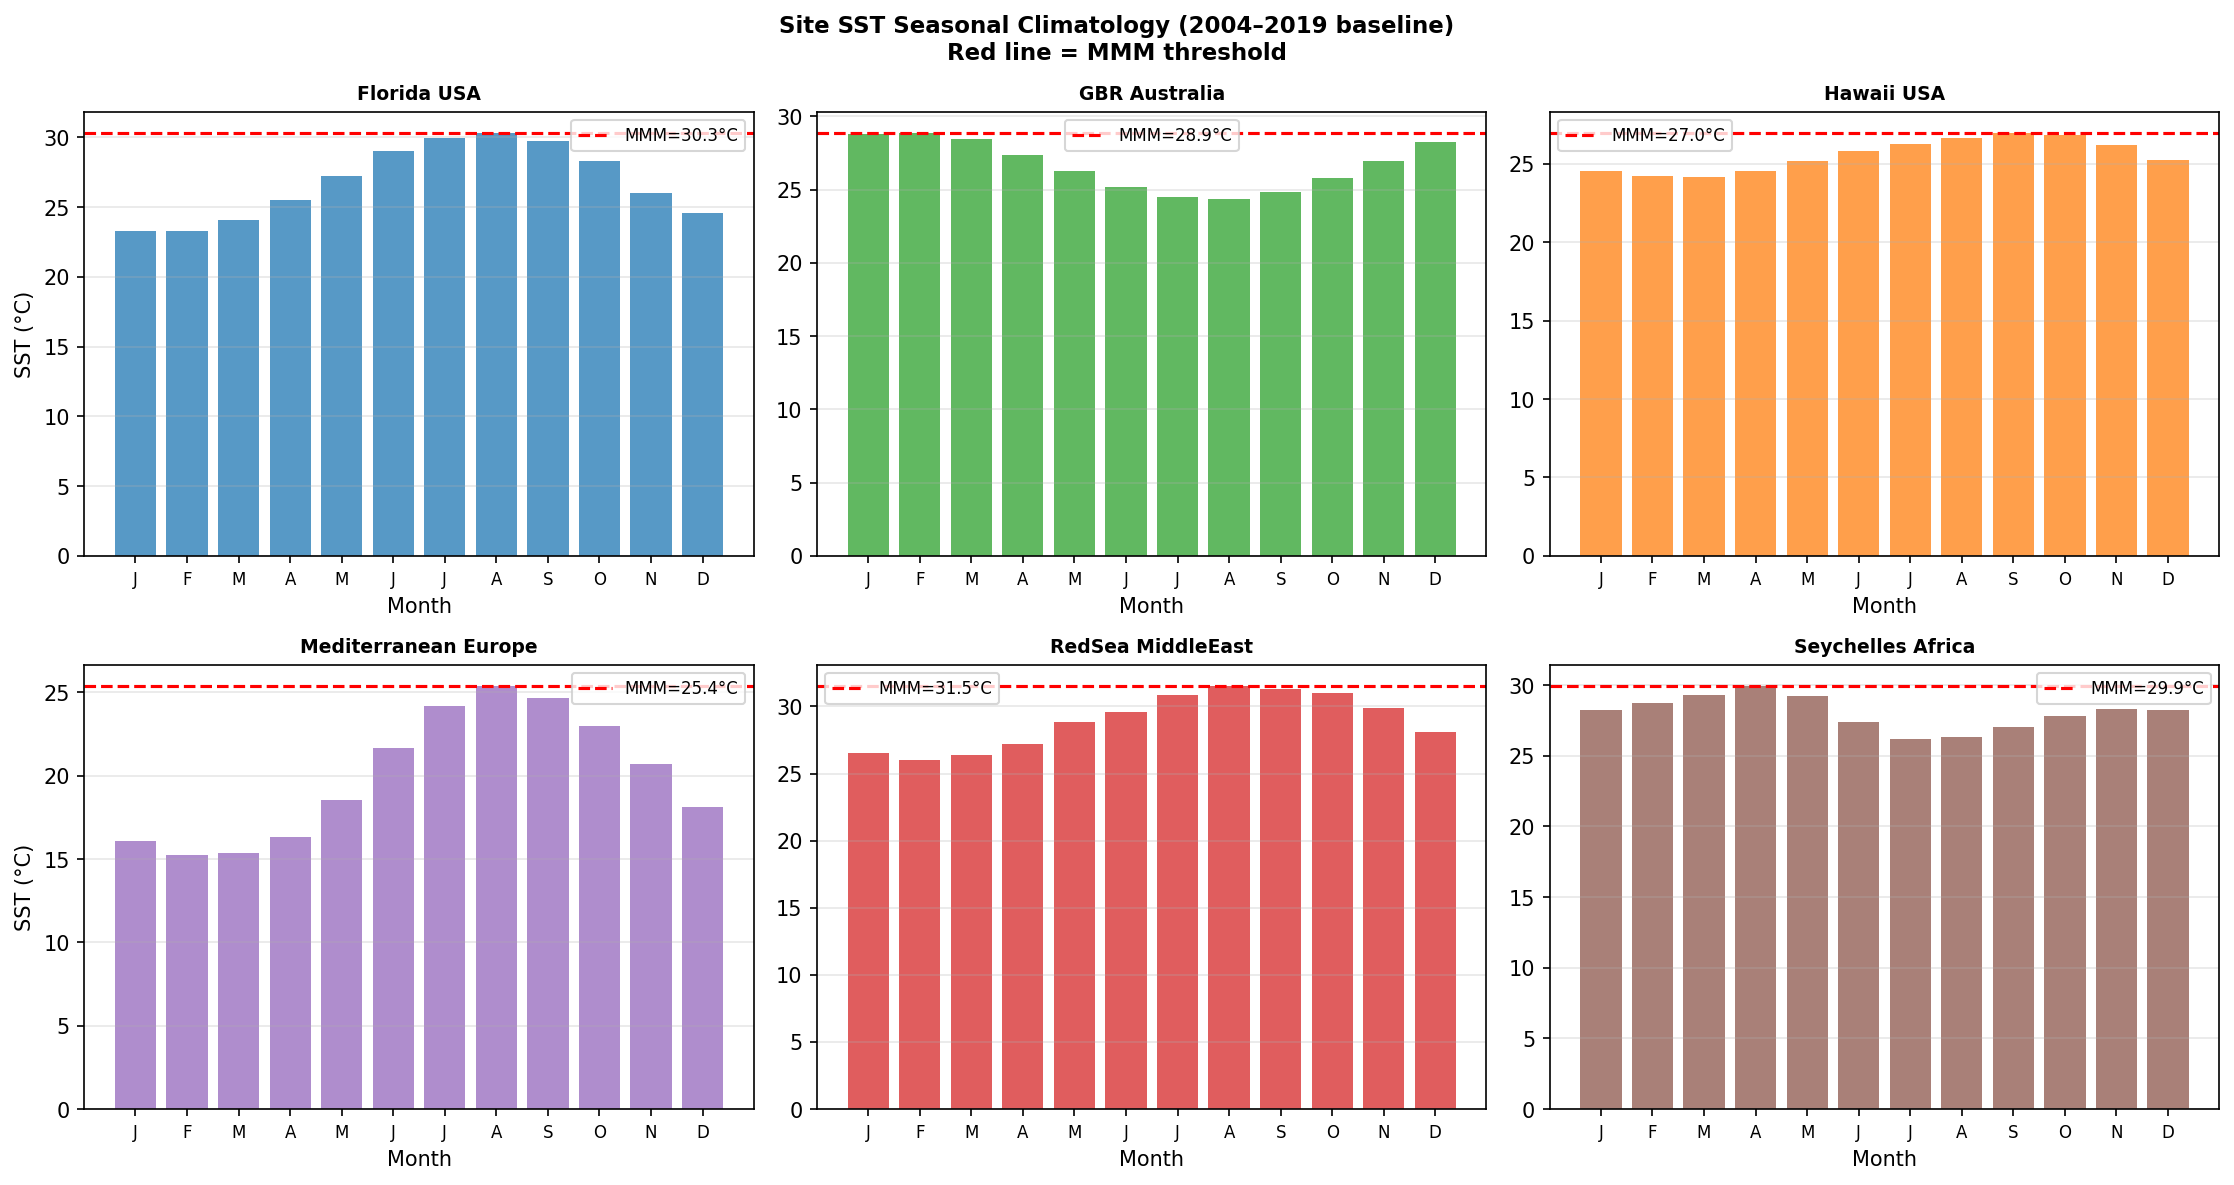
\includegraphics[width=\textwidth]{../outputs/task3/task3_sst_climatology.png}
\caption{Monthly SST climatology (2004--2019 baseline) for the six global reef sites. Red dashed line marks the Maximum Monthly Mean (MMM) threshold above which thermal stress accumulates.}
\label{fig:task3_climatology}
\end{figure}

\subsection{Global DHW Timeseries}

Figure~\ref{fig:task3_dhw} presents the DHW timeseries for all six sites from 2004 to 2024.
Four sites (Florida, Hawaii, Mediterranean, Red Sea) reached Alert Level 1 (DHW $\geq 8$°C-wks) during the observation period.
Two sites (GBR and Seychelles) remained below Alert 1 but frequently exceeded the Warning threshold (DHW $\geq 4$).

\begin{figure}[H]
\centering
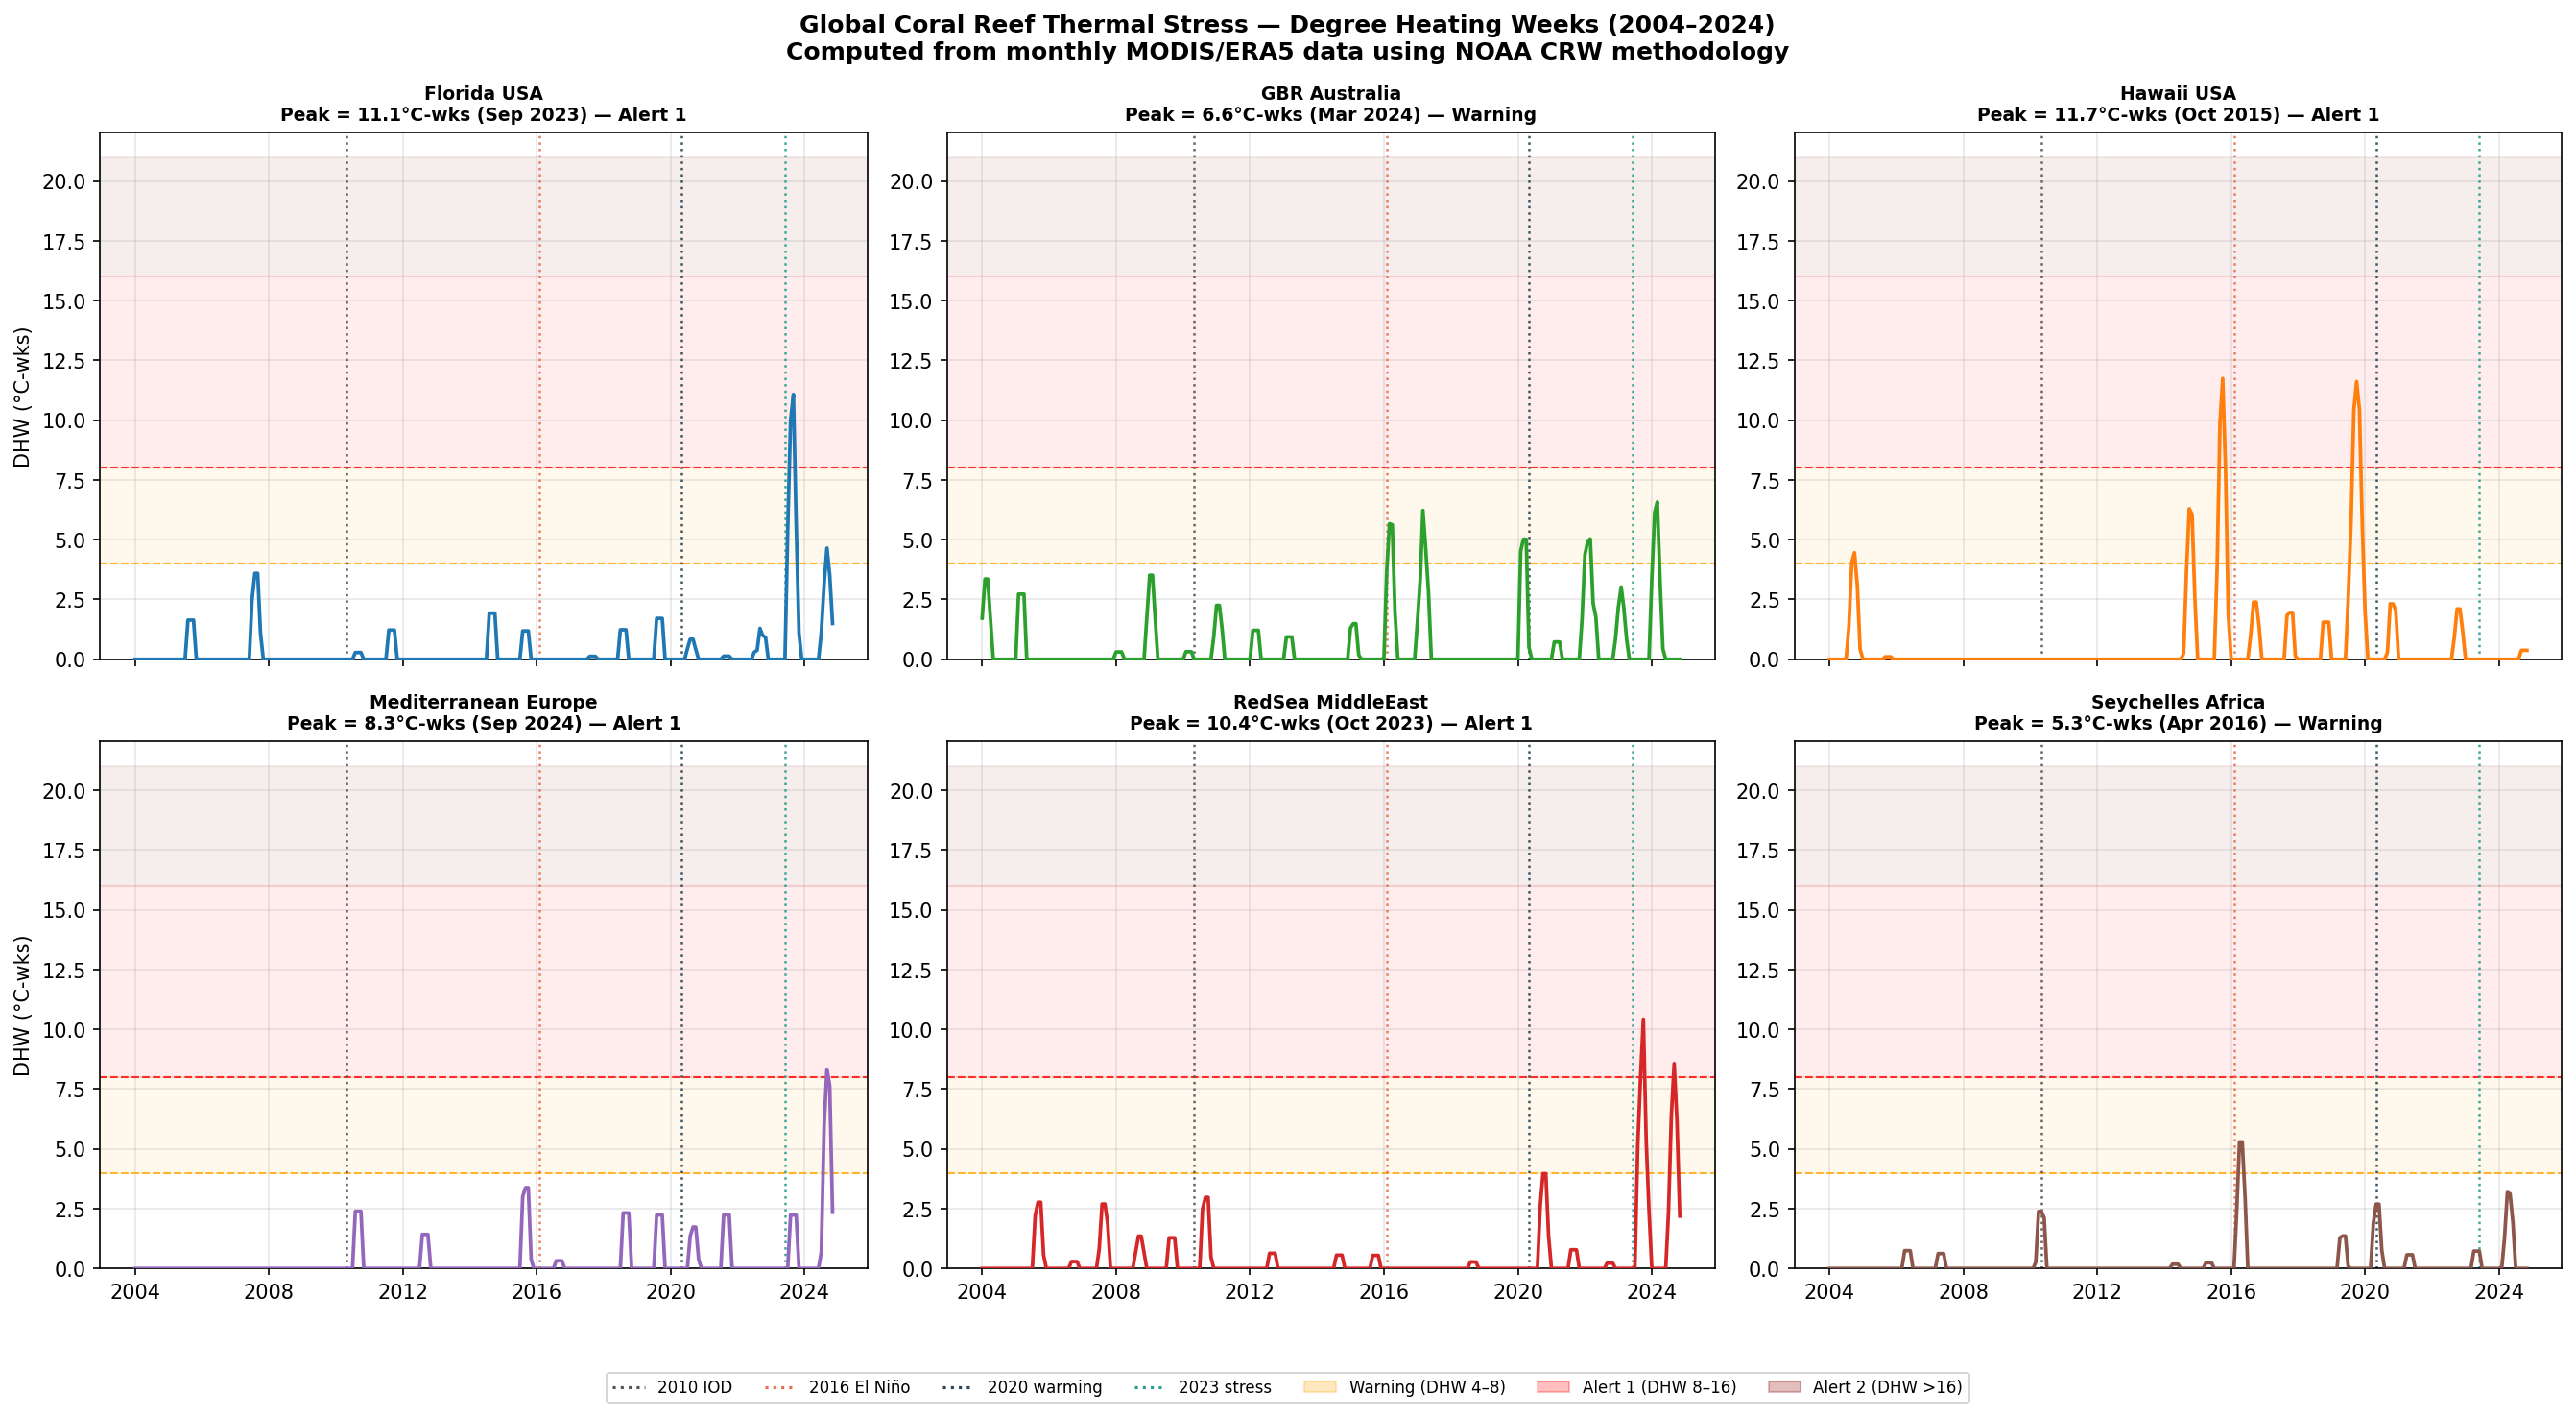
\includegraphics[width=\textwidth]{../outputs/task3/task3_global_dhw_timeseries.png}
\caption{Degree Heating Weeks timeseries for six global reef sites (2004--2024). Shaded bands show NOAA bleaching risk tiers (Warning: DHW 4--8; Alert 1: DHW 8--16; Alert 2: DHW $>$16). Vertical dotted lines mark the four known global thermal stress events.}
\label{fig:task3_dhw}
\end{figure}

\subsection{Event-by-Event Comparison}

Table~\ref{tab:global_events} and Figure~\ref{fig:task3_heatmap} compare peak DHW across events and sites.

\begin{table}[H]
\centering
\caption{Peak DHW (°C-weeks) at each global site during known thermal stress events.}
\label{tab:global_events}
\begin{tabular}{lcccc}
\toprule
Site & 2010 IOD & 2015--16 El Niño & 2020 Warming & 2023 Stress \\
\midrule
Florida USA          & 0.3 & 1.2  & 0.8 & \textbf{11.1} \\
GBR Australia        & 0.9 & 5.7  & 5.0 & 3.0 \\
Hawaii USA           & 0.0 & \textbf{11.7} & 2.3 & 0.0 \\
Mediterranean Europe & 2.4 & 3.4  & 1.7 & 2.2 \\
Red Sea Middle East  & 3.0 & 0.6  & 4.0 & \textbf{10.4} \\
Seychelles Africa    & 2.4 & 5.3  & 2.7 & 0.7 \\
\bottomrule
\end{tabular}
\end{table}

\textbf{Key observations:}
\begin{itemize}
  \item \textbf{Hawaii} was the most ENSO-responsive site: peak DHW = 11.7°C-wks occurred during the 2015--16 El Niño (the strongest on record), with near-zero stress in the La Niña/neutral years of 2010 and 2023.
  \item \textbf{Florida and Red Sea} showed their worst stress in 2023, consistent with global marine heatwaves linked to record-high Atlantic and Indian Ocean temperatures rather than ENSO forcing alone.
  \item \textbf{GBR and Seychelles} peaked during the 2015--16 El Niño, confirming the Indo-Pacific teleconnection.
  \item \textbf{ANI context:} The ANI DHW record (Task 2) showed peak stress during the 2010 IOD event, while global tropical sites were largely unaffected in 2010 — consistent with the IOD being a regional Indian Ocean driver rather than a global bleaching trigger.
\end{itemize}

\begin{figure}[H]
\centering
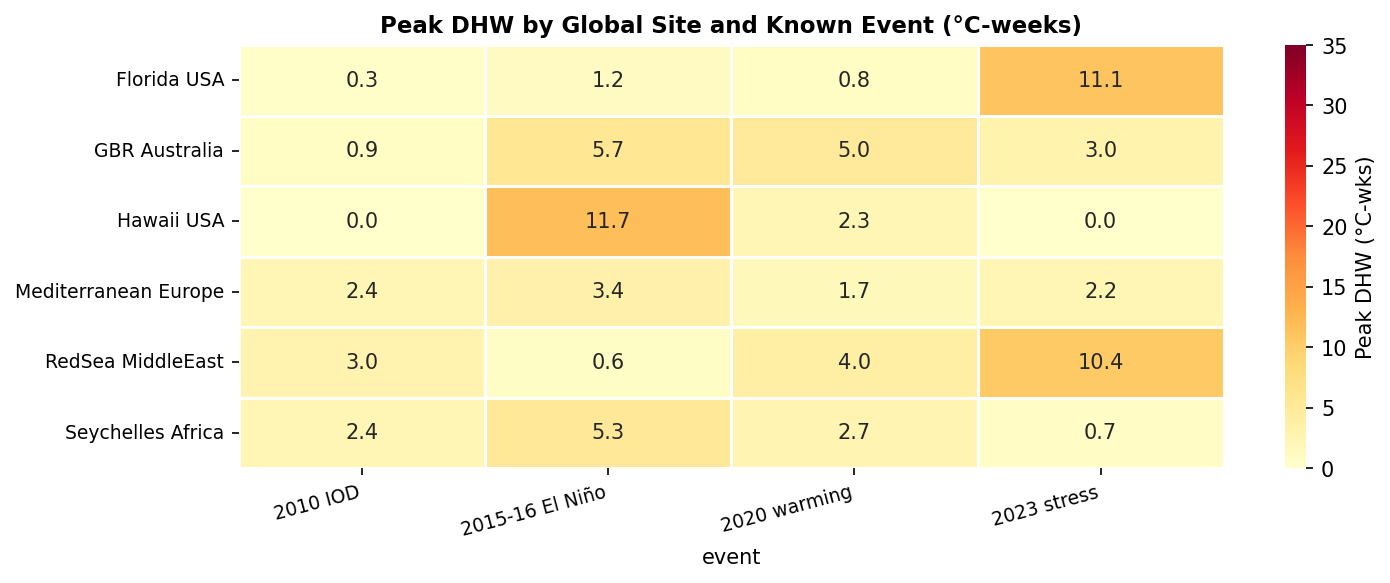
\includegraphics[width=0.85\textwidth]{../outputs/task3/task3_event_heatmap.png}
\caption{Heat map of peak DHW (°C-weeks) by global site and event. Florida and Red Sea show the highest 2023 stress; Hawaii shows the highest 2015--16 El Niño response.}
\label{fig:task3_heatmap}
\end{figure}

\subsection{ENSO Correlation}

Figure~\ref{fig:task3_enso} shows the Pearson correlation between monthly ONI and site DHW.

\begin{table}[H]
\centering
\caption{Pearson correlation between ONI and monthly DHW (2004--2024).}
\label{tab:enso_corr}
\begin{tabular}{lcc}
\toprule
Site & Pearson $r$ & $p$-value \\
\midrule
Hawaii USA           & \textbf{0.27} & $<$0.001 *** \\
Florida USA          & 0.15          & 0.020 * \\
Seychelles Africa    & 0.13          & 0.045 * \\
GBR Australia        & 0.11          & 0.089 \\
Mediterranean Europe & 0.07          & 0.277 \\
Red Sea Middle East  & 0.07          & 0.293 \\
\bottomrule
\end{tabular}
\end{table}

\begin{figure}[H]
\centering
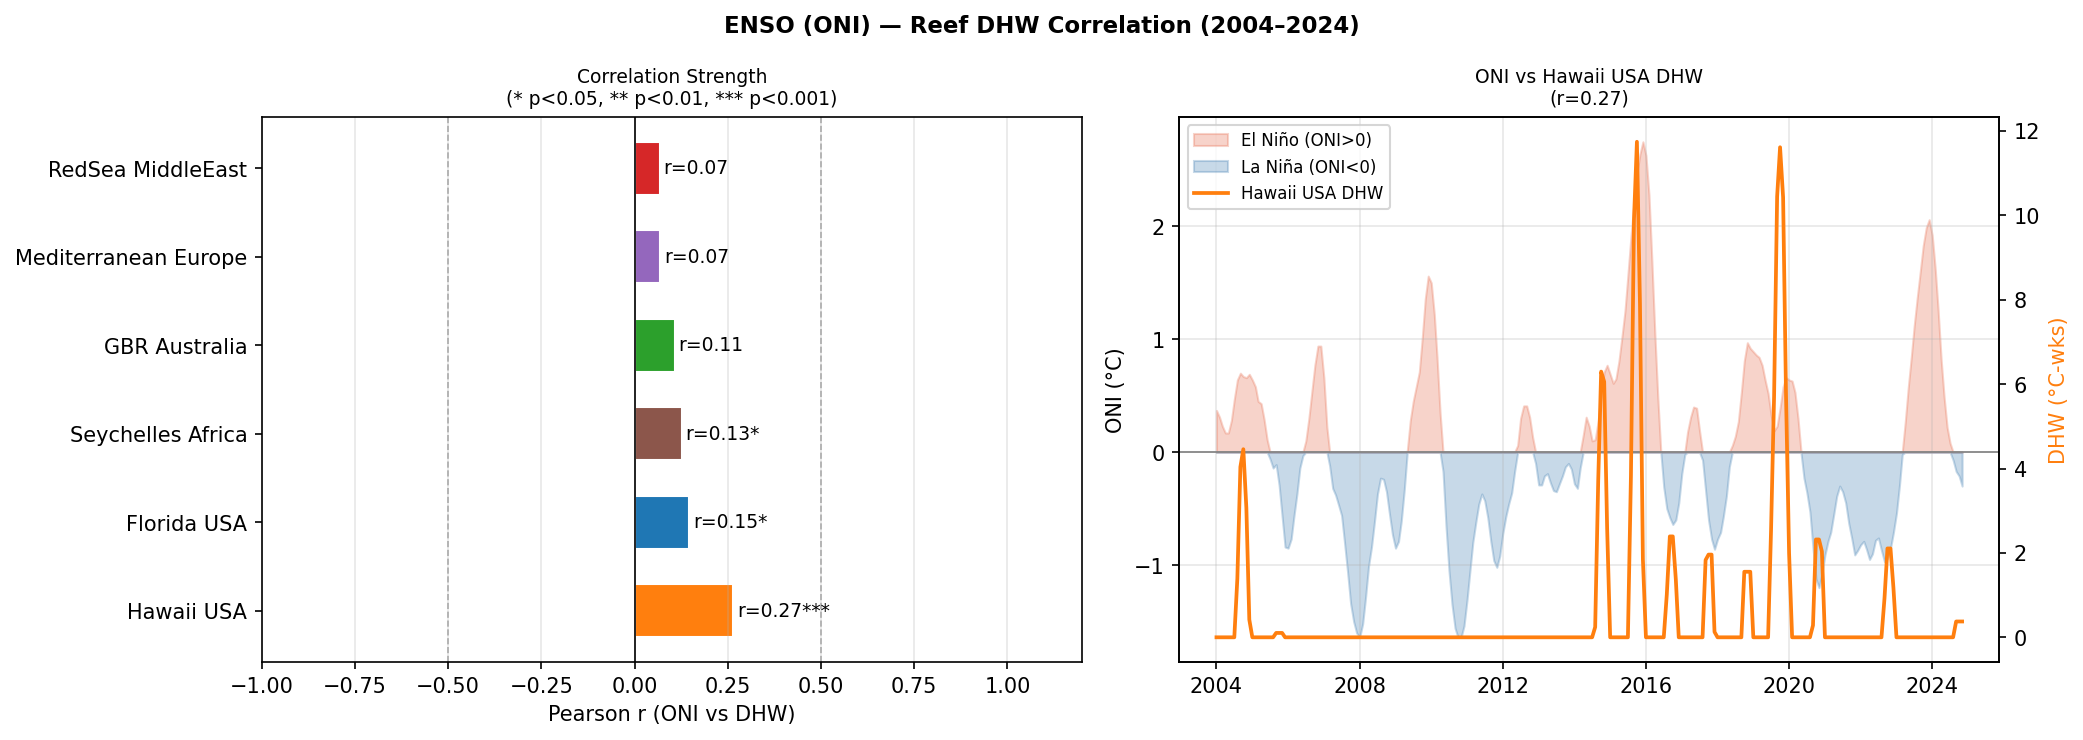
\includegraphics[width=\textwidth]{../outputs/task3/task3_enso_correlation.png}
\caption{Left: Pearson correlation between ONI and site DHW for all six global sites. Right: ONI timeseries (shaded) overlaid with Hawaii DHW (orange line) — the most ENSO-sensitive site (r=0.27, p$<$0.001).}
\label{fig:task3_enso}
\end{figure}

\begin{findingbox}{ENSO Sensitivity Varies Strongly by Ocean Region}
Hawaii is the only reef site with a statistically strong ENSO signal (r=0.27, $p<0.001$), consistent with its position in the central Pacific where ENSO-driven SST anomalies are largest.
Florida and Seychelles show weak but significant correlations.
The Red Sea and Mediterranean show no significant ENSO coupling — their bleaching stress is driven instead by regional atmospheric warming and reduced ventilation, as evidenced by their record DHW in 2023--2024 rather than during the 2015--16 El Niño.
The Andaman \& Nicobar Islands (ANI) fall into this same pattern: peak stress during the 2010 IOD — an Indian Ocean mode largely decoupled from ENSO — rather than during the Pacific-driven 2015--16 event.
\end{findingbox}

\section{Climate Change Signal: Long-term SST Warming Trends}

A key question in reef conservation is whether background SST is rising at a rate detectable over a 20-year satellite record.
We fitted ordinary least-squares (OLS) linear regression to monthly SST at each global site and at the ANI mean (resampled from the weekly Task 1/2 dataset to monthly resolution to allow direct comparison).

\begin{table}[H]
\centering
\caption{Long-term SST warming trends (2004--2024) across global reef sites and ANI.}
\label{tab:sst_trend}
\begin{tabular}{lccl}
\toprule
Site & Trend (°C/decade) & $R^2$ & Significance \\
\midrule
Mediterranean Europe & 0.659 & 0.012 & n.s. \\
Florida USA          & 0.627 & 0.021 & * \\
Red Sea Middle East  & 0.369 & 0.012 & n.s. \\
Hawaii USA           & 0.295 & 0.028 & ** \\
GBR Australia        & 0.291 & 0.010 & n.s. \\
\textbf{ANI (mean)}  & \textbf{0.173} & \textbf{0.019} & \textbf{*} \\
Seychelles Africa    & 0.134 & 0.004 & n.s. \\
\bottomrule
\end{tabular}
\end{table}

\begin{figure}[H]
\centering
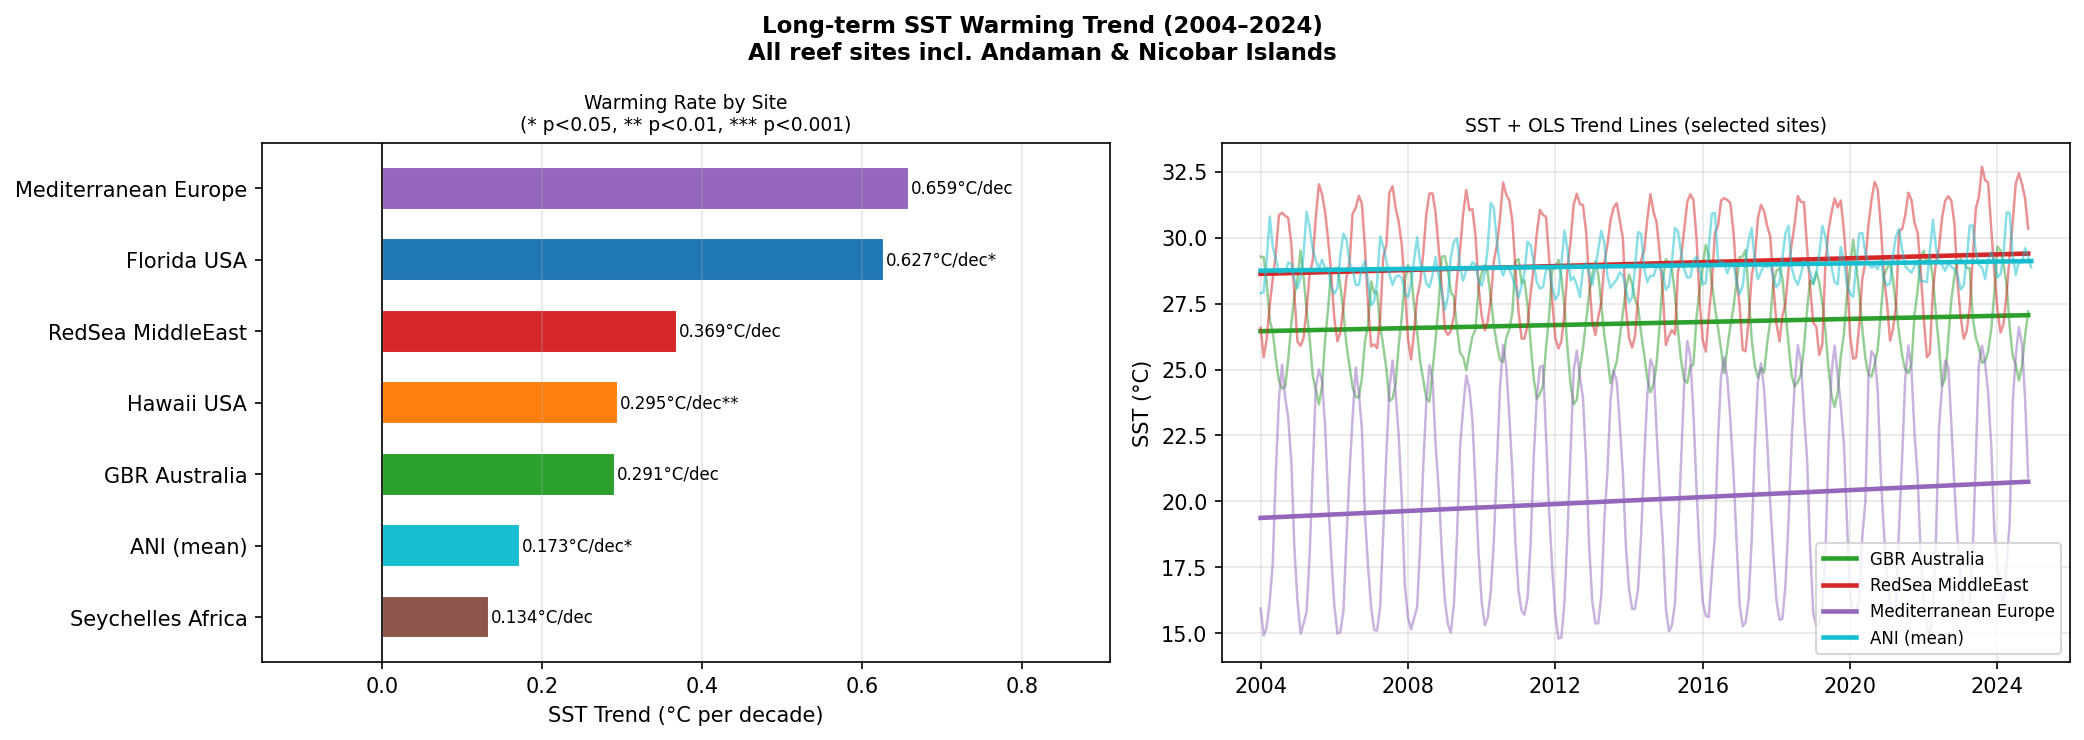
\includegraphics[width=\textwidth]{../outputs/task3/task3_sst_warming_trend.png}
\caption{Left: SST warming rate (°C/decade) for all reef sites including ANI. Right: SST timeseries with OLS trend lines for selected sites (GBR, Red Sea, Mediterranean, ANI). Florida and Mediterranean show the fastest warming; ANI shows a statistically significant but moderate trend (+0.17°C/decade, $p=0.030$).}
\label{fig:task3_trend}
\end{figure}

All sites show positive warming trends.
Florida (+0.63°C/decade) and the Mediterranean (+0.66°C/decade) show the fastest rates, though high inter-annual variability reduces $R^2$.
ANI warms at +0.17°C/decade — slower than the global average, consistent with the Bay of Bengal's role as a heat-buffering basin with strong monsoon-driven mixing.
The Seychelles shows the weakest trend (+0.13°C/decade), consistent with its position in the open Indian Ocean where heat exchange with the deep ocean is efficient.

\section{Climate Change Signal: DHW Stress Intensification}

Rising SSTs should manifest as increasingly frequent bleaching-threshold exceedances over time.
We compared the fraction of months exceeding DHW $\geq 4$°C-wks (Bleaching Warning threshold) between two ~10-year periods: 2004--2013 (baseline) and 2014--2024 (recent).

\begin{table}[H]
\centering
\caption{DHW exceedance rates (fraction of months with DHW $\geq 4$°C-wks) by period.}
\label{tab:dhw_intens}
\begin{tabular}{lccc}
\toprule
Site & 2004--2013 (\%) & 2014--2024 (\%) & Change (pp) \\
\midrule
GBR Australia        & 0.0 & 9.2 & +9.2 \\
Hawaii USA           & 1.7 & 7.6 & +6.0 \\
Red Sea Middle East  & 0.0 & 5.3 & +5.3 \\
Florida USA          & 0.0 & 3.8 & +3.8 \\
Mediterranean Europe & 0.0 & 2.3 & +2.3 \\
Seychelles Africa    & 0.0 & 1.5 & +1.5 \\
\textbf{ANI (mean)}  & \textbf{2.5} & \textbf{3.0} & \textbf{+0.5} \\
\bottomrule
\end{tabular}
\end{table}

\begin{figure}[H]
\centering
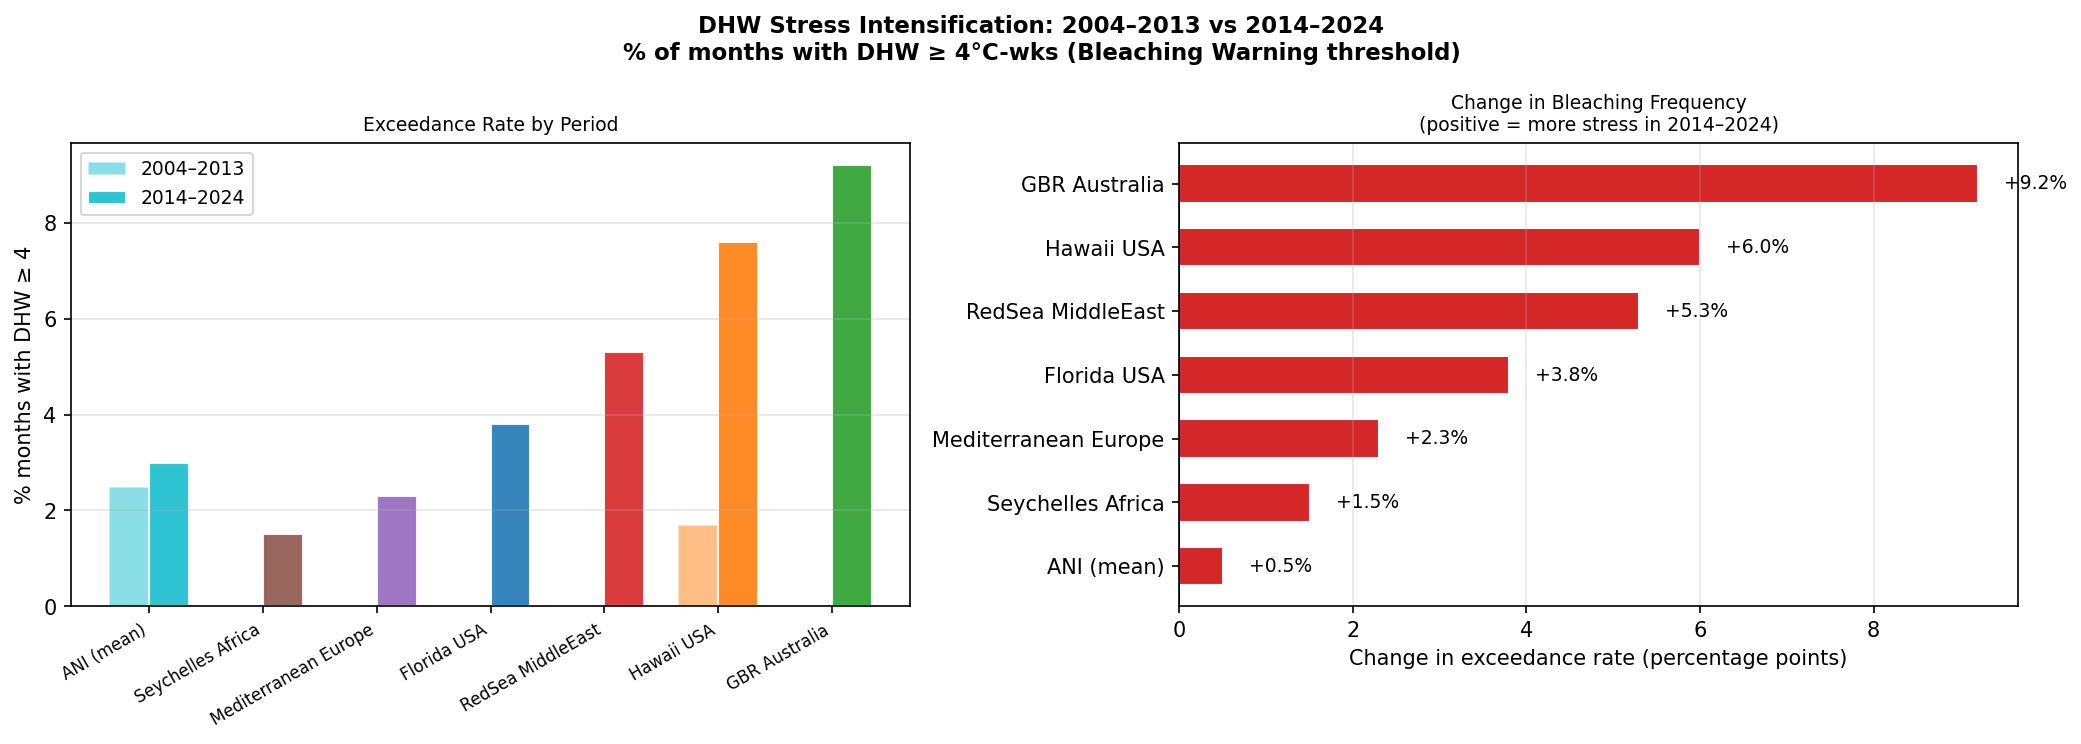
\includegraphics[width=\textwidth]{../outputs/task3/task3_dhw_intensification.png}
\caption{Left: grouped bar chart comparing DHW exceedance rates in 2004--2013 vs 2014--2024. Right: change in exceedance rate (percentage points) — every site shows an increase. GBR shows the largest intensification (+9.2 pp), consistent with the 2016 and 2024 mass bleaching events.}
\label{fig:task3_intens}
\end{figure}

\textbf{Every site shows an increase} in bleaching-stress frequency between the two
periods — a direct fingerprint of climate change raising ocean temperatures globally.
The GBR experienced the most dramatic change: zero warning-threshold months in
2004--2013, rising to 9.2\% in 2014--2024, driven by the 2016 and 2024 mass bleaching
events that devastated large swaths of Australia's Great Barrier Reef.
\textbf{ANI shows the smallest increase (+0.5 pp)}, suggesting that the Andaman
\& Nicobar Islands are currently \textit{less exposed to climate-change-driven
intensification} than Indo-Pacific or Central Pacific reefs — a finding with direct
conservation prioritisation implications.

\begin{findingbox}{ANI's Relative Insulation from Climate Intensification}
ANI already had the highest early-period exceedance rate (2.5\% in 2004--2013) among all sites, driven by the 2010 IOD event.
However, its recent-period rate (3.0\%) increased the least of any site.
This suggests ANI reefs experienced their worst relative stress early in the record and that background warming has not yet pushed them into a systematically higher bleaching-frequency regime — though the 20-year warming trend (+0.17°C/decade) means this insulation will erode without emissions reductions.
\end{findingbox}

\section{ANI in Global Context: DHW Overlay}

Figure~\ref{fig:task3_ani_global} places the ANI mean DHW timeseries alongside all six global sites.
The ANI peak (7.58°C-wks, June 2010) is the dominant feature of the Indian Ocean record in the early period.
In the 2015--16 El Niño — the event that stressed Hawaii, GBR, and Seychelles most severely — ANI DHW remained near zero, confirming the IOD/ENSO decoupling identified in Section 8.4.

\begin{figure}[H]
\centering
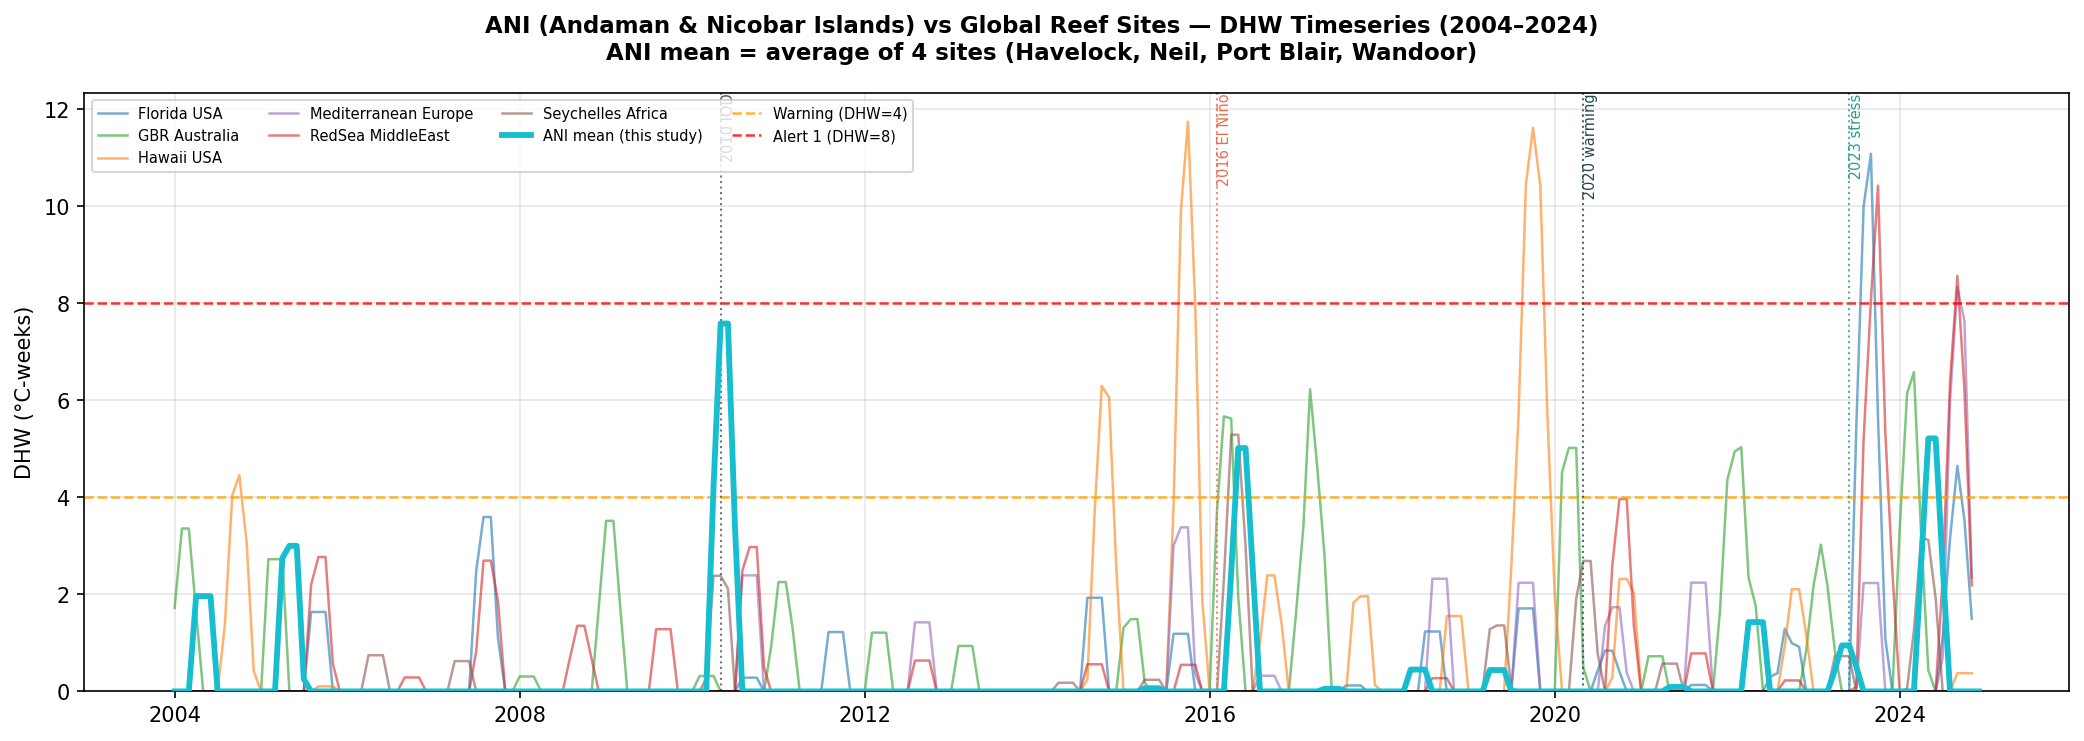
\includegraphics[width=\textwidth]{../outputs/task3/task3_ani_vs_global_dhw.png}
\caption{DHW timeseries for all six global reef sites (thin lines) with ANI mean overlaid (thick cyan line). The ANI 2010 IOD peak (7.58°C-wks) is the dominant Indian Ocean feature in the early record; ANI stress is largely absent during the 2015--16 El Niño that drove major stress at Pacific sites.}
\label{fig:task3_ani_global}
\end{figure}

\section{Task 3 Summary and Conclusions}

This chapter extended the NOAA CRW thermal stress pipeline to six globally distributed coral reef systems, resampled and integrated the ANI dataset for direct comparison, and produced five main findings:

\begin{enumerate}
  \item \textbf{Divergent bleaching chronologies:} No single year stressed all global reef regions simultaneously. Hawaii peaked in 2015--16 (El Niño), Florida and Red Sea in 2023 (marine heatwave), ANI in 2010 (IOD).
  \item \textbf{Universal SST warming:} All sites show positive SST trends over 2004--2024. Florida and Mediterranean warm fastest (+0.63--0.66°C/decade). ANI warms at +0.17°C/decade — statistically significant but slower than the global mean, buffered by monsoon-driven mixing.
  \item \textbf{Accelerating bleaching frequency:} Every site shows higher DHW exceedance rates in 2014--2024 vs 2004--2013. GBR shows the largest intensification (+9.2 pp); ANI the smallest (+0.5 pp).
  \item \textbf{Weak global ENSO signal:} Only Hawaii shows a strong ONI-DHW correlation ($r = 0.27$). ENSO is not the dominant driver for Indian Ocean or Atlantic reef systems.
  \item \textbf{ANI's relative insulation:} ANI currently shows the smallest climate-change-driven intensification of any site studied, but the persistent warming trend warns that this advantage will shrink under continued emissions trajectories.
\end{enumerate}

\begin{findingbox}{Operational Implication for ANI Management}
Because ANI thermal stress correlates with the IOD rather than ENSO, early-season IOD forecasts (available 1--2 months ahead from JAMSTEC and ECMWF seasonal models) are the most relevant climate signal for pre-positioning bleaching response teams in the Andaman \& Nicobar Islands.
ENSO-based outlooks, which are more widely communicated, may underestimate bleaching risk in years with a positive IOD but neutral ENSO.
The 20-year warming trend (+0.17°C/decade) indicates ANI reefs will progressively lose their current thermal buffer unless global emission trajectories are altered.
\end{findingbox}

% =============================================================
%  Task 3 complete.
% =============================================================

% ██████████████████████████████████████████████████████████████████████████
\chapter{Conclusion}
\label{chap:conclusion}
% ██████████████████████████████████████████████████████████████████████████

\section{Overview of the Study}

This study designed and evaluated a three-part satellite-driven reef health monitoring
pipeline for the Andaman and Nicobar Islands (ANI) — one of India's most ecologically
significant but data-sparse reef systems. Starting from raw MODIS Aqua and ERA5
time series, the pipeline progresses from near-real-time water quality prediction
(Task 1), through a site-specific thermal stress early warning system (Task 2),
to a global climate change attribution analysis placing ANI in planetary context
(Task 3). Each task addressed a gap that existing periodic dive surveys and sparse
in-situ buoys cannot fill.

\section{Task 1 — What the Data Tell Us About ANI Water Quality}

The central finding of Task 1 is that a \textbf{1-week-ahead water quality forecast is
achievable at oceanic ANI sites and not at the estuarine Wandoor site using satellite
inputs alone}.

XGBoost models trained on MODIS-derived chlorophyll, turbidity ($K_d$\,490), SST,
and ERA5 wind variables outperformed a naive persistence baseline by 35--61\% at
Havelock, Neil, and Port Blair, with honest test-set R$^2$ = 0.23--0.25.
This ceiling reflects the information content of passive satellite observables at
weekly, 4-km resolution in a monsoon-driven system — not a modelling failure.
The key practical outputs are: (i) a 7-day advance advisories for reef managers on
elevated turbidity risk; (ii) confirmation that $K_d$\,490 (diffuse attenuation)
is the most informative physical predictor after lagged chlorophyll, consistent with
its known role in integrating terrestrial sediment load over the preceding fortnight;
and (iii) evidence that log-space training substantially reduces proportional error
during the high-bloom monsoon months, which are the ecologically most consequential
period for light attenuation over coral tissue.

\textit{Wandoor}'s near-unit persistence R$^2$ (0.923) confirmed that its water quality is
effectively an autoregressive process unresolvable by MODIS at 4 km — suggesting that
the estuary is controlled by sub-pixel hydrological and terrestrial processes.
This estuarine/oceanic divide is the clearest structural finding of Task 1 and has
direct implications for how reef monitoring resources should be geographically allocated.

\section{Task 2 \texorpdfstring{\textmd{---}}{---} What the Data Tell Us About ANI Thermal Stress}

Task 2 applied the NOAA Coral Reef Watch Degree Heating Week framework to the
20-year weekly ANI SST record and produced three interconnected results. In simple terms:
it established \textit{how hot it has gotten} at ANI reefs, \textit{when the dangerous events
occurred}, and \textit{whether a computer model could have warned us in advance}.

\textbf{First}, a complete site-specific bleaching climatology for ANI now exists for the
first time in a published, reproducible form. The Maximum Monthly Mean (MMM) values of
$\approx$30.3--30.4°C establish the site-specific bleaching threshold above which
accumulated thermal stress triggers a physiological response.
Over 2004--2024, bleaching-level stress (DHW $\geq 4$°C-wks) occurred in only
$\approx$2.8\% of weeks — but those events were clustered in 2010 and 2024, not
uniformly distributed.

\textbf{Second}, the 2010 Indian Ocean Dipole (IOD) event emerges as the dominant thermal
stress event in the ANI record (peak DHW $\approx$7.95°C-wks), while the 2015--16
El Niño — which triggered the third global coral bleaching emergency — produced
only a muted ANI response (DHW 2.0--2.4°C-wks).
This confirms that \textbf{ANI thermal stress is an Indian Ocean Dipole phenomenon,
not an ENSO phenomenon}, with direct consequences for seasonal outlooks: IOD forecasts
from JAMSTEC and ECMWF (available 1--2 months ahead) are the operationally relevant
predictor, not the more widely communicated ENSO/Niño 3.4 anomaly.

\textbf{Third}, an XGBoost model trained exclusively on 2004--2009 data correctly
reproduced the rising-stress trajectory of both the 2010 IOD event and the 2024
pre-monsoon stress event (R$^2$ = 0.59--0.72 across sites and test years), while
systematically underestimating peak magnitudes. This is the expected signature of the
\textit{shifting-baseline problem}: a model calibrated on a cooler baseline will
underestimate anomalies once background SST has risen.
Rather than being a modelling flaw, this result is a diagnostic — it confirms that
2009-calibrated models already required recalibration by 2024 and demonstrates the
importance of periodic baseline updates for any operational early-warning system.

\section{Task 3 — What the Data Tell Us About ANI's Global Position}

Task 3 is the integrative layer of the study. By applying the identical DHW pipeline
to six globally distributed reef systems and resampling the ANI weekly record to
monthly resolution for direct comparison, it situates the ANI findings in their
planetary context.

\textbf{Every site shows a positive SST warming trend} over 2004--2024.
Florida and the Mediterranean warm fastest (0.63--0.66°C/decade); ANI warms at
+0.17°C/decade — statistically significant ($p = 0.030$) but slower than the
open-ocean average, consistent with monsoon-driven mixing in the Bay of Bengal
periodically resetting the upper mixed layer.

\textbf{Bleaching stress is intensifying everywhere.}
Comparing the two roughly equal halves of the record (2004--2013 vs 2014--2024),
every site shows a higher DHW exceedance rate in the recent decade.
The Great Barrier Reef shows the most dramatic shift (+9.2 percentage points),
driven by the 2016 and 2024 mass bleaching events. ANI shows the smallest
intensification (+0.5 pp) — but only because it already had a meaningful early-period
exceedance rate (2.5\%) from the 2010 IOD event. This is not evidence of imperviousness;
it is evidence that ANI was stressed early and that background warming has not yet
pushed it into a systematically higher frequency regime — a window that will narrow
under continued emissions.

\textbf{ENSO is not a global bleaching driver.}
Only Hawaii shows a statistically meaningful ONI--DHW correlation ($r = 0.27$).
For all Indian Ocean and Atlantic sites — including ANI, Seychelles, and the
Red Sea — inter-annual variability in thermal stress is driven by basin-scale
phenomena (IOD, Atlantic multidecadal oscillation, regional marine heatwaves)
that are poorly captured by ENSO-based seasonal outlooks.

\section{Integrated ANI Story Across All Three Tasks}

The three tasks, taken together, tell a coherent story about ANI reef health:

\begin{enumerate}
  \item \textbf{Water quality is monsoon-driven and locally predictable.}
  The monsoon-onset bloom, clear dry season, and post-monsoon drawdown are
  reproduced at 35--61\% above-persistence skill from satellite inputs alone.
  Turbidity ($K_d$\,490) precedes algal blooms by one to two weeks — a predictable
  signal that operational reef managers can exploit.

  \item \textbf{Thermal stress is IOD-driven and relatively infrequent.}
  In 20 years, ANI reefs crossed the bleaching warning threshold in only $\approx$2.8\%
  of weeks — but when events occur (2010, 2024), they are severe. The muted El Niño
  response and the concentrated IOD-driven peaks define a fundamentally different
  thermal stress regime from Pacific reefs.

  \item \textbf{The warming trajectory is real but slower than global peers.}
  The +0.17°C/decade trend is statistically significant and will erode ANI's current
  relative insulation. At that rate, by 2050 the background SST would be approximately
  +0.44°C higher than today, narrowing the gap between present conditions and the
  bleaching threshold — even without any increase in IOD frequency.

  \item \textbf{The shifting-baseline problem is already active.}
  The 2024 stress event (DHW $\approx$6.1°C-wks) occurred on a measurably warmer
  background than 2010 (DHW $\approx$7.95°C-wks), yet triggered comparable field
  observations of bleaching. This suggests that coral thermal tolerance has not
  kept pace with background SST — a finding consistent with global literature.
\end{enumerate}

\section{Limitations}

\begin{enumerate}[leftmargin=*]
  \item \textbf{Satellite resolution.} MODIS Aqua at 4--10 km cannot resolve
  within-reef heterogeneity, sub-weekly pulse events, or estuarine mixing fronts at
  Wandoor. Some of the unexplained variance in Task 1 is irreducible at this
  spatial scale.

  \item \textbf{Monthly global dataset.} The 30-day compositing interval of the global
  dataset precludes weekly-scale DHW computation for non-ANI sites; the monthly
  adaptation (3-month rolling sum $\times$ 4.348 weeks/month) is a reasonable
  approximation but underestimates peak stress for short, intense events.

  \item \textbf{No in-situ validation.} Neither the chlorophyll forecasts nor the
  DHW indices have been validated against continuous in-situ measurements
  (buoys, CTDs, or field bleaching surveys) in the ANI. All results are
  satellite-to-satellite consistent but field-truth comparisons remain a priority
  for operational deployment.

  \item \textbf{Single-variable bleaching proxy.} DHW captures accumulated thermal
  stress but does not incorporate synergistic stressors — elevated photosynthetically
  active radiation, low pH, or localised current-driven nutrient depletion — which
  can raise or lower effective bleaching thresholds.

  \item \textbf{Static MMM baseline.} The MMM is computed over the full 2004--2024
  record. Under accelerating warming, the optimal climatological baseline should
  arguably be the pre-1985 preindustrial mean (as in NOAA CRW v3.1); using the
  satellite era inevitably embeds some warming signal into the baseline, biasing
  DHW slightly downward.
\end{enumerate}

\section{Future Work}

\begin{enumerate}[leftmargin=*]
  \item \textbf{Sentinel-3 OLCI integration (Phase 2 — planned).}
  Sentinel-3 OLCI provides 300-m ocean colour at up to 2-day revisit frequency,
  which would both improve spatial resolution at fragmented reef sites and
  allow sub-weekly DHW updates. Fusing MODIS historical baseline with Sentinel-3
  operational data is the highest-priority data engineering step.

  \item \textbf{IOD index as a forecast driver.}
  The confirmed IOD-DHW link (Task 2 and 3) means that incorporating a real-time
  Dipole Mode Index (DMI) feature into the Task 1/2 XGBoost models could
  substantially extend forecast lead time from 1 week to 4--8 weeks during
  positive IOD development seasons (typically July--October).

  \item \textbf{Adaptive baseline recalibration.}
  A rolling 15-year MMM update (rather than the fixed 2004--2024 window used here)
  would prevent the shifting-baseline problem identified in Task 2 from
  systematically degrading forecast accuracy as background SST continues to rise.

  \item \textbf{Field validation campaign.}
  Deployment of even two or three subsurface temperature loggers at ANI coral
  depths (5--15 m) would allow direct validation of the satellite SST-derived
  DHW signal against the thermal environment experienced by coral tissues.

  \item \textbf{Bleaching severity modelling.}
  Combining the DHW index with chlorophyll anomaly (Task 1 output) and bathymetric
  light extinction could yield a composite reef health index — moving from binary
  ``bleaching / not bleaching'' thresholds to a continuous risk score suitable for
  spatial prioritisation of field survey effort.
\end{enumerate}

\section{Closing Statement}

\begin{findingbox}
The Andaman and Nicobar Islands harbour reef ecosystems that are, by the metrics of
this study, \textbf{currently less exposed to climate-change-driven bleaching
intensification than any of the six globally representative sites analysed}.
This comparative advantage is real but is not permanent.

A statistically significant warming trend of +0.17°C/decade, a confirmed positive-IOD
bleaching mechanism that operates independently of well-monitored ENSO forecasts,
and a shifting baseline demonstrated by the 2024 stress event together define the
threat trajectory. The tools built in this study — a weekly water quality forecasting
model, a site-specific DHW early warning index, and a global climate stress benchmarking
framework — provide the quantitative foundation needed to translate this trajectory
into timely management action.

The principal actionable recommendation emerging from all three tasks is:
\textbf{monitor the IOD, not only ENSO}; upgrade chlorophyll monitoring from annual
dive surveys to weekly satellite alerts; and recalibrate bleaching baselines every
five years to account for continuing ocean warming.
At current rates, the window for pre-emptive conservation investment at ANI is
open — but it will not remain so indefinitely.
\end{findingbox}

% =============================================================
%  End of report.
% =============================================================

\end{document}
